\documentclass[tikz,crop,convert={density=200,outext=.png},border=0.4cm]{standalone}

\usepackage{pgfplots}
\usepackage{amsmath}
\usetikzlibrary{arrows.meta}
\usepackage{physics}
\usepackage{xcolor}
\definecolor{pow_1}{RGB}{103,0,31}
\definecolor{pow_2}{RGB}{206,18,86}
\definecolor{pow_3}{RGB}{223,101,176}
\pgfplotsset{compat=newest,
    %width=6cm,
    %height=3cm,
    scale only axis=true,
    max space between ticks=25pt,
    try min ticks=5,
    every axis/.style={
        axis y line=middle,
        axis x line=middle,
        axis line style={thick,->,>=latex, shorten >=-.3cm}
    },
    every axis plot/.append style={thick},
    tick style={black, thick},
}
\tikzset{
    semithick/.style={line width=0.8pt},
}
\usepgfplotslibrary{groupplots}
\usepgfplotslibrary{dateplot}
% Document begins
\begin{document}
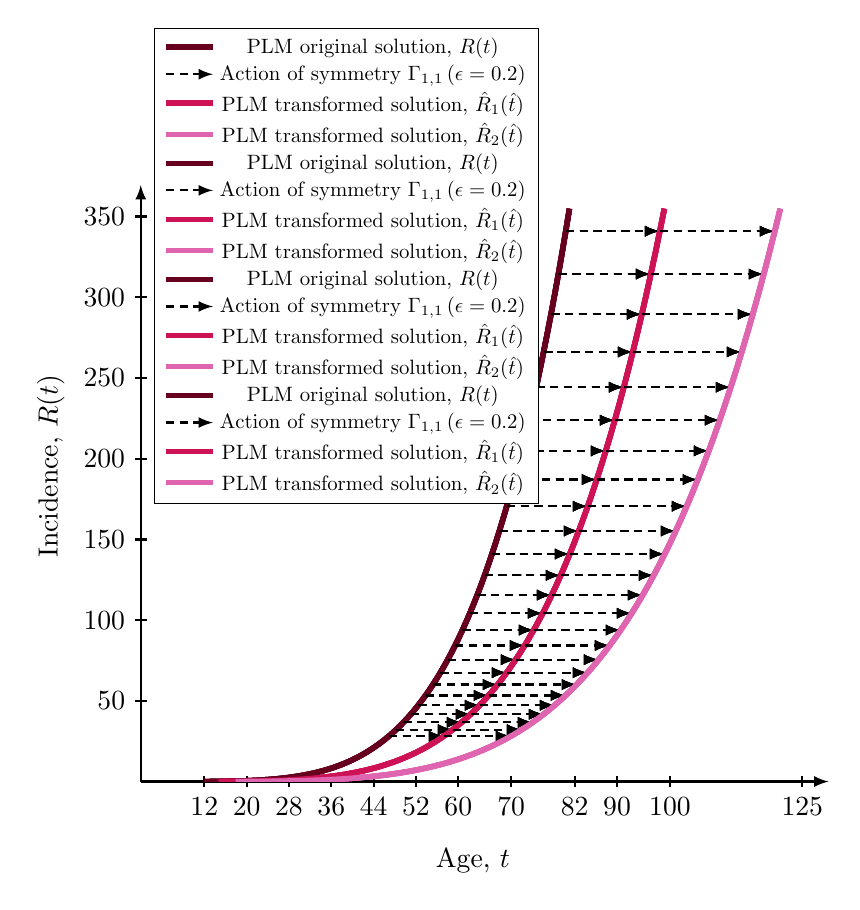
\begin{tikzpicture}
  % The axis of the plot
\begin{axis}[
    %title={Model: $\dv{y}{t}=\frac{2y}{t}$ with solution $y(t)=C_1t^2$\\Symmetry: $\Gamma_{\epsilon}=(t,y)\mapsto\left(\exp\left(\epsilon\right)t,\exp\left(-\epsilon\right)y\right)$},
    title style = {align=left},
    xlabel={Age, $t$},
    ylabel={Incidence, $R(t)$},
    %ylabel={Logarithm of Incidence, $\ln\left(R(t)\right)$},        
    x label style={at={(axis description cs:0.5,-0.1)},anchor=north},
    y label style={at={(axis description cs:-0.1,0.55)},rotate=90,anchor=south},    
    xmin=0, xmax=125.5,
    % xmin=-27, xmax=5,
    %ymin=-20, ymax=20,
    %xtick={-30,-27,...,9},
    xtick={0,12,20,...,60,70,82,90,100,125},    
    %ytick={-15,-10,...,15},
    legend style={at={(axis description cs:0.02,0.9)},anchor=west,nodes={scale=0.75, transform shape}},    
    %legend pos=north west,
    %ymajorgrids=true,
    grid style=dashed,
]
% Plot the data
%\input{./Input/PLM_t_a.tex}
%\input{./Input/PLM_t_b.tex}
%\input{./Input/PLM_t_c.tex}
%\input{./Input/PLM_t_d.tex}
\addplot[
color=pow_1,line width=2pt,
]
coordinates {%
(12.0,0.051142608117798666)
(12.696969696969697,0.06642780291034586)
(13.393939393939394,0.08508372113063335)
(14.09090909090909,0.10761896101053291)
(14.787878787878789,0.13458718503595257)
(15.484848484848484,0.16658858817033514)
(16.18181818181818,0.20427133954061952)
(16.87878787878788,0.24833299928646488)
(17.575757575757578,0.2995219120931209)
(18.272727272727273,0.35863857877401645)
(18.96969696969697,0.426537007136173)
(19.666666666666668,0.5041260432462906)
(20.363636363636363,0.5923706841148557)
(21.060606060606062,0.6922933727274928)
(21.757575757575758,0.8049752762751438)
(22.454545454545453,0.931557548365929)
(23.151515151515152,1.0732425759404736)
(23.84848484848485,1.2312952115579283)
(24.545454545454547,1.407043991671122)
(25.242424242424242,1.6018823414652514)
(25.93939393939394,1.8172697667951332)
(26.636363636363637,2.054733033719942)
(27.333333333333336,2.3158673361020647)
(28.03030303030303,2.602337451707067)
(28.727272727272727,2.915878887214675)
(29.424242424242426,3.258299012526224)
(30.12121212121212,3.631478184731217)
(30.81818181818182,4.03737086207495)
(31.515151515151516,4.478006708250098)
(32.21212121212122,4.955491687317427)
(32.90909090909091,5.472009149544508)
(33.60606060606061,6.0298209084364585)
(34.303030303030305,6.6312683092181715)
(35.0,7.278773289015399)
(35.6969696969697,7.974839428969067)
(36.39393939393939,8.722052998506346)
(37.09090909090909,9.523083991981913)
(37.78787878787879,10.380687157891877)
(38.484848484848484,11.297703020855138)
(39.18181818181819,12.277058896546698)
(39.87878787878788,13.321769899761337)
(40.57575757575758,14.43493994577601)
(41.27272727272727,15.619762745175155)
(41.96969696969697,16.879522792293056)
(42.66666666666667,18.217596347424532)
(43.36363636363637,19.637452412945997)
(44.06060606060606,21.14265370348628)
(44.75757575757576,22.736857610278854)
(45.45454545454545,24.423817159823038)
(46.151515151515156,26.20738196697801)
(46.84848484848485,28.09149918260661)
(47.54545454545455,30.08021443588455)
(48.24242424242424,32.177672771382994)
(48.939393939393945,34.38811958103263)
(49.63636363636364,36.715901531069875)
(50.333333333333336,39.165467484066404)
(51.03030303030303,41.741369416133864)
(51.72727272727273,44.44826332940154)
(52.42424242424243,47.29091015985039)
(53.121212121212125,50.274176680594955)
(53.81818181818182,53.40303640069465)
(54.515151515151516,56.68257045957432)
(55.21212121212122,60.11796851713643)
(55.909090909090914,63.714529639637)
(56.60606060606061,67.47766318140152)
(57.303030303030305,71.41288966245361)
(58.0,75.52584164212143)
(58.6969696969697,79.82226458869494)
(59.3939393939394,84.30801774519647)
(60.09090909090909,88.98907499132832)
(60.78787878787879,93.87152570166137)
(61.48484848484849,98.96157560012223)
(62.18181818181819,104.26554761084031)
(62.87878787878788,109.78988270540843)
(63.57575757575758,115.54114074661764)
(64.27272727272728,121.52600132871441)
(64.96969696969697,127.75126461423507)
(65.66666666666667,134.22385216747358)
(66.36363636363637,140.95080778462128)
(67.06060606060606,147.9392983206405)
(67.75757575757576,155.19661451290835)
(68.45454545454547,162.73017180168645)
(69.15151515151516,170.54751114745136)
(69.84848484848484,178.65629984513882)
(70.54545454545455,187.0643323353423)
(71.24242424242425,195.77953101250293)
(71.93939393939394,204.80994703013835)
(72.63636363636364,214.1637611031492)
(73.33333333333334,223.8492843072355)
(74.03030303030303,233.87495887547115)
(74.72727272727273,244.24935899206656)
(75.42424242424244,254.98119158336306)
(76.12121212121212,266.07929710608425)
(76.81818181818183,277.5526503328825)
(77.51515151515152,289.41036113523444)
(78.21212121212122,301.6616752636771)
(78.9090909090909,314.3159751254626)
(79.60606060606061,327.3827805596266)
(80.30303030303031,340.87174960953456)
(81.0,354.7926792929032)
};
\addlegendentry{PLM original solution, $R(t)$}
\addplot[
color=black,->,>=latex,densely dashed
]
coordinates {%
(46.84848484848485,28.09149918260661)
(47.790107770911824,28.09149918260661)
(48.750656678478066,28.09149918260661)
(49.73051197070972,28.09149918260661)
(50.73006169290663,28.09149918260661)
(51.74970168981723,28.09149918260661)
(52.78983576240219,28.09149918260661)
(53.85087582774895,28.09149918260661)
(54.93324208220033,28.09149918260661)
(56.037363167762024,28.09149918260661)
(57.163676341854696,28.09149918260661)
};
\addlegendentry{Action of symmetry $\Gamma_{1,1}\left(\epsilon=0.2\right)$}
\addplot[
forget plot,
color=black,->,>=latex,densely dashed
]
coordinates {%
(48.24242424242424,32.177672771382994)
(49.21206440575137,32.177672771382994)
(50.201193681848046,32.177672771382994)
(51.210203788725664,32.177672771382994)
(52.23949431766323,32.177672771382994)
(53.289472891454736,32.177672771382994)
(54.36055532583718,32.177672771382994)
(55.45316579416321,32.177672771382994)
(56.56773699538352,32.177672771382994)
(57.70471032540565,32.177672771382994)
(58.86453605189694,32.177672771382994)
};
\addplot[
forget plot,
color=black,->,>=latex,densely dashed
]
coordinates {%
(49.63636363636364,36.715901531069875)
(50.63402104059092,36.715901531069875)
(51.65173068521803,36.715901531069875)
(52.6898956067416,36.715901531069875)
(53.74892694241983,36.715901531069875)
(54.82924409309224,36.715901531069875)
(55.931274889272174,36.715901531069875)
(57.05545576057747,36.715901531069875)
(58.20223190856671,36.715901531069875)
(59.37205748304928,36.715901531069875)
(60.56539576193919,36.715901531069875)
};
\addplot[
forget plot,
color=black,->,>=latex,densely dashed
]
coordinates {%
(51.03030303030303,41.741369416133864)
(52.05597767543047,41.741369416133864)
(53.10226768858801,41.741369416133864)
(54.169587424757545,41.741369416133864)
(55.25835956717643,41.741369416133864)
(56.369015294729756,41.741369416133864)
(57.50199445270717,41.741369416133864)
(58.65774572699174,41.741369416133864)
(59.836726821749906,41.741369416133864)
(61.039404640692915,41.741369416133864)
(62.266255471981445,41.741369416133864)
};
\addplot[
forget plot,
color=black,->,>=latex,densely dashed
]
coordinates {%
(52.42424242424243,47.29091015985039)
(53.47793431027002,47.29091015985039)
(54.552804691957995,47.29091015985039)
(55.649279242773495,47.29091015985039)
(56.76779219193304,47.29091015985039)
(57.90878649636728,47.29091015985039)
(59.07271401614217,47.29091015985039)
(60.26003569340601,47.29091015985039)
(61.4712217349331,47.29091015985039)
(62.70675179833655,47.29091015985039)
(63.96711518202369,47.29091015985039)
};
\addplot[
forget plot,
color=black,->,>=latex,densely dashed
]
coordinates {%
(53.81818181818182,53.40303640069465)
(54.89989094510957,53.40303640069465)
(56.00334169532797,53.40303640069465)
(57.12897106078943,53.40303640069465)
(58.27722481668963,53.40303640069465)
(59.44855769800478,53.40303640069465)
(60.643433579577156,53.40303640069465)
(61.86232565982026,53.40303640069465)
(63.10571664811628,53.40303640069465)
(64.37409895598016,53.40303640069465)
(65.66797489206593,53.40303640069465)
};
\addplot[
forget plot,
color=black,->,>=latex,densely dashed
]
coordinates {%
(55.21212121212122,60.11796851713643)
(56.32184757994912,60.11796851713643)
(57.453878698697956,60.11796851713643)
(58.608662878805376,60.11796851713643)
(59.78665744144623,60.11796851713643)
(60.98832889964229,60.11796851713643)
(62.214153143012155,60.11796851713643)
(63.464615626234526,60.11796851713643)
(64.74021156129947,60.11796851713643)
(66.0414461136238,60.11796851713643)
(67.36883460210818,60.11796851713643)
};
\addplot[
forget plot,
color=black,->,>=latex,densely dashed
]
coordinates {%
(56.60606060606061,67.47766318140152)
(57.74380421478867,67.47766318140152)
(58.90441570206793,67.47766318140152)
(60.08835469682131,67.47766318140152)
(61.29609006620283,67.47766318140152)
(62.5281001012798,67.47766318140152)
(63.78487270644714,67.47766318140152)
(65.06690559264878,67.47766318140152)
(66.37470647448266,67.47766318140152)
(67.70879327126742,67.47766318140152)
(69.06969431215042,67.47766318140152)
};
\addplot[
forget plot,
color=black,->,>=latex,densely dashed
]
coordinates {%
(58.0,75.52584164212143)
(59.165760849628214,75.52584164212143)
(60.35495270543791,75.52584164212143)
(61.568046514837256,75.52584164212143)
(62.80552269095943,75.52584164212143)
(64.06787130291731,75.52584164212143)
(65.35559226988214,75.52584164212143)
(66.66919555906306,75.52584164212143)
(68.00920138766587,75.52584164212143)
(69.37614042891107,75.52584164212143)
(70.77055402219268,75.52584164212143)
};
\addplot[
forget plot,
color=black,->,>=latex,densely dashed
]
coordinates {%
(59.3939393939394,84.30801774519647)
(60.58771748446777,84.30801774519647)
(61.8054897088079,84.30801774519647)
(63.04773833285321,84.30801774519647)
(64.31495531571603,84.30801774519647)
(65.60764250455482,84.30801774519647)
(66.92631183331713,84.30801774519647)
(68.27148552547732,84.30801774519647)
(69.64369630084906,84.30801774519647)
(71.0434875865547,84.30801774519647)
(72.47141373223494,84.30801774519647)
};
\addplot[
forget plot,
color=black,->,>=latex,densely dashed
]
coordinates {%
(60.78787878787879,93.87152570166137)
(62.00967411930731,93.87152570166137)
(63.25602671217787,93.87152570166137)
(64.52743015086914,93.87152570166137)
(65.82438794047263,93.87152570166137)
(67.14741370619234,93.87152570166137)
(68.49703139675213,93.87152570166137)
(69.87377549189159,93.87152570166137)
(71.27819121403226,93.87152570166137)
(72.71083474419834,93.87152570166137)
(74.17227344227719,93.87152570166137)
};
\addplot[
forget plot,
color=black,->,>=latex,densely dashed
]
coordinates {%
(62.18181818181819,104.26554761084031)
(63.431630754146866,104.26554761084031)
(64.70656371554786,104.26554761084031)
(66.00712196888509,104.26554761084031)
(67.33382056522923,104.26554761084031)
(68.68718490782985,104.26554761084031)
(70.06775096018713,104.26554761084031)
(71.47606545830585,104.26554761084031)
(72.91268612721545,104.26554761084031)
(74.37818190184197,104.26554761084031)
(75.87313315231944,104.26554761084031)
};
\addplot[
forget plot,
color=black,->,>=latex,densely dashed
]
coordinates {%
(63.57575757575758,115.54114074661764)
(64.85358738898641,115.54114074661764)
(66.15710071891783,115.54114074661764)
(67.48681378690102,115.54114074661764)
(68.84325318998583,115.54114074661764)
(70.22695610946735,115.54114074661764)
(71.6384705236221,115.54114074661764)
(73.0783554247201,115.54114074661764)
(74.54718104039863,115.54114074661764)
(76.04552905948559,115.54114074661764)
(77.57399286236168,115.54114074661764)
};
\addplot[
forget plot,
color=black,->,>=latex,densely dashed
]
coordinates {%
(64.96969696969697,127.75126461423507)
(66.27554402382596,127.75126461423507)
(67.6076377222878,127.75126461423507)
(68.96650560491696,127.75126461423507)
(70.35268581474243,127.75126461423507)
(71.76672731110486,127.75126461423507)
(73.2091900870571,127.75126461423507)
(74.68064539113436,127.75126461423507)
(76.18167595358182,127.75126461423507)
(77.7128762171292,127.75126461423507)
(79.27485257240392,127.75126461423507)
};
\addplot[
forget plot,
color=black,->,>=latex,densely dashed
]
coordinates {%
(66.36363636363637,140.95080778462128)
(67.69750065866552,140.95080778462128)
(69.0581747256578,140.95080778462128)
(70.44619742293293,140.95080778462128)
(71.86211843949906,140.95080778462128)
(73.3064985127424,140.95080778462128)
(74.77990965049212,140.95080778462128)
(76.28293535754865,140.95080778462128)
(77.81617086676503,140.95080778462128)
(79.38022337477287,140.95080778462128)
(80.9757122824462,140.95080778462128)
};
\addplot[
forget plot,
color=black,->,>=latex,densely dashed
]
coordinates {%
(67.75757575757576,155.19661451290835)
(69.11945729350506,155.19661451290835)
(70.50871172902778,155.19661451290835)
(71.92588924094885,155.19661451290835)
(73.37155106425563,155.19661451290835)
(74.84626971437987,155.19661451290835)
(76.35062921392708,155.19661451290835)
(77.88522532396289,155.19661451290835)
(79.4506657799482,155.19661451290835)
(81.04757053241647,155.19661451290835)
(82.6765719924884,155.19661451290835)
};
\addplot[
forget plot,
color=black,->,>=latex,densely dashed
]
coordinates {%
(69.15151515151516,170.54751114745136)
(70.54141392834461,170.54751114745136)
(71.95924873239775,170.54751114745136)
(73.40558105896478,170.54751114745136)
(74.88098368901223,170.54751114745136)
(76.3860409160174,170.54751114745136)
(77.92134877736208,170.54751114745136)
(79.48751529037716,170.54751114745136)
(81.0851606931314,170.54751114745136)
(82.7149176900601,170.54751114745136)
(84.37743170253066,170.54751114745136)
};
\addplot[
forget plot,
color=black,->,>=latex,densely dashed
]
coordinates {%
(70.54545454545455,187.0643323353423)
(71.96337056318416,187.0643323353423)
(73.40978573576774,187.0643323353423)
(74.88527287698074,187.0643323353423)
(76.39041631376884,187.0643323353423)
(77.92581211765491,187.0643323353423)
(79.49206834079709,187.0643323353423)
(81.08980525679144,187.0643323353423)
(82.7196556063146,187.0643323353423)
(84.38226484770375,187.0643323353423)
(86.07829141257292,187.0643323353423)
};
\addplot[
forget plot,
color=black,->,>=latex,densely dashed
]
coordinates {%
(71.93939393939394,204.80994703013835)
(73.3853271980237,204.80994703013835)
(74.86032273913771,204.80994703013835)
(76.36496469499667,204.80994703013835)
(77.89984893852542,204.80994703013835)
(79.4655833192924,204.80994703013835)
(81.06278790423207,204.80994703013835)
(82.69209522320568,204.80994703013835)
(84.35415051949778,204.80994703013835)
(86.04961200534737,204.80994703013835)
(87.77915112261516,204.80994703013835)
};
\addplot[
forget plot,
color=black,->,>=latex,densely dashed
]
coordinates {%
(73.33333333333334,223.8492843072355)
(74.80728383286326,223.8492843072355)
(76.3108597425077,223.8492843072355)
(77.84465651301262,223.8492843072355)
(79.40928156328204,223.8492843072355)
(81.00535452092993,223.8492843072355)
(82.63350746766706,223.8492843072355)
(84.29438518961993,223.8492843072355)
(85.98864543268095,223.8492843072355)
(87.71695916299097,223.8492843072355)
(89.48001083265738,223.8492843072355)
};
\addplot[
forget plot,
color=black,->,>=latex,densely dashed
]
coordinates {%
(74.72727272727273,244.24935899206656)
(76.22924046770282,244.24935899206656)
(77.7613967458777,244.24935899206656)
(79.32434833102859,244.24935899206656)
(80.91871418803866,244.24935899206656)
(82.54512572256746,244.24935899206656)
(84.20422703110208,244.24935899206656)
(85.89667515603423,244.24935899206656)
(87.62314034586419,244.24935899206656)
(89.38430632063465,244.24935899206656)
(91.18087054269968,244.24935899206656)
};
\addplot[
forget plot,
color=black,->,>=latex,densely dashed
]
coordinates {%
(76.12121212121212,266.07929710608425)
(77.65119710254237,266.07929710608425)
(79.21193374924768,266.07929710608425)
(80.80404014904452,266.07929710608425)
(82.42814681279526,266.07929710608425)
(84.08489692420497,266.07929710608425)
(85.77494659453707,266.07929710608425)
(87.49896512244848,266.07929710608425)
(89.25763525904736,266.07929710608425)
(91.05165347827827,266.07929710608425)
(92.88173025274192,266.07929710608425)
};
\addplot[
forget plot,
color=black,->,>=latex,densely dashed
]
coordinates {%
(77.51515151515152,289.41036113523444)
(79.07315373738192,289.41036113523444)
(80.66247075261765,289.41036113523444)
(82.28373196706045,289.41036113523444)
(83.93757943755183,289.41036113523444)
(85.62466812584246,289.41036113523444)
(87.34566615797205,289.41036113523444)
(89.10125508886273,289.41036113523444)
(90.89213017223054,289.41036113523444)
(92.71900063592187,289.41036113523444)
(94.58258996278414,289.41036113523444)
};
\addplot[
forget plot,
color=black,->,>=latex,densely dashed
]
coordinates {%
(78.9090909090909,314.3159751254626)
(80.49511037222146,314.3159751254626)
(82.11300775598762,314.3159751254626)
(83.76342378507638,314.3159751254626)
(85.44701206230843,314.3159751254626)
(87.16443932747997,314.3159751254626)
(88.91638572140704,314.3159751254626)
(90.70354505527699,314.3159751254626)
(92.52662508541373,314.3159751254626)
(94.3863477935655,314.3159751254626)
(96.28344967282639,314.3159751254626)
};
\addplot[
forget plot,
color=black,->,>=latex,densely dashed
]
coordinates {%
(80.30303030303031,340.87174960953456)
(81.91706700706102,340.87174960953456)
(83.56354475935763,340.87174960953456)
(85.24311560309235,340.87174960953456)
(86.95644468706506,340.87174960953456)
(88.7042105291175,340.87174960953456)
(90.48710528484206,340.87174960953456)
(92.30583502169128,340.87174960953456)
(94.16111999859694,340.87174960953456)
(96.05369495120917,340.87174960953456)
(97.98430938286866,340.87174960953456)
};
\addplot[
color=pow_2,line width=2pt,
]
coordinates {%
(14.65683309792204,0.051142608117798666)
(15.508113808154885,0.06642780291034586)
(16.35939451838773,0.08508372113063335)
(17.210675228620573,0.10761896101053291)
(18.061955938853423,0.13458718503595257)
(18.913236649086265,0.16658858817033514)
(19.76451735931911,0.20427133954061952)
(20.615798069551957,0.24833299928646488)
(21.467078779784806,0.2995219120931209)
(22.31835949001765,0.35863857877401645)
(23.169640200250495,0.426537007136173)
(24.02092091048334,0.5041260432462906)
(24.872201620716186,0.5923706841148557)
(25.723482330949032,0.6922933727274928)
(26.57476304118188,0.8049752762751438)
(27.42604375141472,0.931557548365929)
(28.27732446164757,1.0732425759404736)
(29.12860517188042,1.2312952115579283)
(29.979885882113262,1.407043991671122)
(30.831166592346104,1.6018823414652514)
(31.682447302578954,1.8172697667951332)
(32.5337280128118,2.054733033719942)
(33.38500872304465,2.3158673361020647)
(34.23628943327749,2.602337451707067)
(35.087570143510334,2.915878887214675)
(35.93885085374318,3.258299012526224)
(36.790131563976026,3.631478184731217)
(37.641412274208875,4.03737086207495)
(38.49269298444172,4.478006708250098)
(39.34397369467457,4.955491687317427)
(40.1952544049074,5.472009149544508)
(41.04653511514026,6.0298209084364585)
(41.8978158253731,6.6312683092181715)
(42.74909653560594,7.278773289015399)
(43.6003772458388,7.974839428969067)
(44.451657956071635,8.722052998506346)
(45.302938666304485,9.523083991981913)
(46.15421937653733,10.380687157891877)
(47.00550008677017,11.297703020855138)
(47.856780797003026,12.277058896546698)
(48.70806150723587,13.321769899761337)
(49.55934221746871,14.43493994577601)
(50.41062292770156,15.619762745175155)
(51.2619036379344,16.879522792293056)
(52.11318434816725,18.217596347424532)
(52.964465058400094,19.637452412945997)
(53.815745768632944,21.14265370348628)
(54.667026478865786,22.736857610278854)
(55.51830718909863,24.423817159823038)
(56.36958789933148,26.20738196697801)
(57.22086860956433,28.09149918260661)
(58.07214931979717,30.08021443588455)
(58.92343003003001,32.177672771382994)
(59.77471074026286,34.38811958103263)
(60.62599145049571,36.715901531069875)
(61.47727216072855,39.165467484066404)
(62.328552870961396,41.741369416133864)
(63.17983358119424,44.44826332940154)
(64.03111429142709,47.29091015985039)
(64.88239500165993,50.274176680594955)
(65.73367571189279,53.40303640069465)
(66.58495642212563,56.68257045957432)
(67.43623713235847,60.11796851713643)
(68.28751784259131,63.714529639637)
(69.13879855282417,67.47766318140152)
(69.99007926305701,71.41288966245361)
(70.84135997328985,75.52584164212143)
(71.6926406835227,79.82226458869494)
(72.54392139375555,84.30801774519647)
(73.3952021039884,88.98907499132832)
(74.24648281422124,93.87152570166137)
(75.0977635244541,98.96157560012223)
(75.94904423468694,104.26554761084031)
(76.80032494491978,109.78988270540843)
(77.65160565515262,115.54114074661764)
(78.50288636538548,121.52600132871441)
(79.3541670756183,127.75126461423507)
(80.20544778585116,134.22385216747358)
(81.056728496084,140.95080778462128)
(81.90800920631685,147.9392983206405)
(82.7592899165497,155.19661451290835)
(83.61057062678255,162.73017180168645)
(84.46185133701539,170.54751114745136)
(85.31313204724822,178.65629984513882)
(86.16441275748107,187.0643323353423)
(87.01569346771393,195.77953101250293)
(87.86697417794676,204.80994703013835)
(88.71825488817962,214.1637611031492)
(89.56953559841247,223.8492843072355)
(90.4208163086453,233.87495887547115)
(91.27209701887816,244.24935899206656)
(92.12337772911101,254.98119158336306)
(92.97465843934384,266.07929710608425)
(93.8259391495767,277.5526503328825)
(94.67721985980953,289.41036113523444)
(95.52850057004238,301.6616752636771)
(96.37978128027522,314.3159751254626)
(97.23106199050807,327.3827805596266)
(98.08234270074092,340.87174960953456)
(98.93362341097375,354.7926792929032)
};
\addlegendentry{PLM transformed solution, $\hat{R}_1(\hat{t})$}
\addplot[
forget plot,
color=black,->,>=latex,densely dashed
]
coordinates {%
(57.22086860956433,28.09149918260661)
(58.37096944416347,28.09149918260661)
(59.54418652921262,28.09149918260661)
(60.740984485742196,28.09149918260661)
(61.96183727335173,28.09149918260661)
(63.20722837790876,28.09149918260661)
(64.47765100302041,28.09149918260661)
(65.77360826535339,28.09149918260661)
(67.0956133938798,28.09149918260661)
(68.44418993312766,28.09149918260661)
(69.81987195051659,28.09149918260661)
};
\addplot[
forget plot,
color=black,->,>=latex,densely dashed
]
coordinates {%
(58.92343003003001,32.177672771382994)
(60.10775119994064,32.177672771382994)
(61.315876425942086,32.177672771382994)
(62.548284153493896,32.177672771382994)
(63.80546244448638,32.177672771382994)
(65.08790917052441,32.177672771382994)
(66.39613221009604,32.177672771382994)
(67.73064964970412,32.177672771382994)
(69.0919899890405,32.177672771382994)
(70.48069235028409,32.177672771382994)
(71.89730669160568,32.177672771382994)
};
\addplot[
forget plot,
color=black,->,>=latex,densely dashed
]
coordinates {%
(60.62599145049571,36.715901531069875)
(61.844532955717824,36.715901531069875)
(63.08756632267158,36.715901531069875)
(64.35558382124562,36.715901531069875)
(65.64908761562104,36.715901531069875)
(66.96858996314006,36.715901531069875)
(68.31461341717167,36.715901531069875)
(69.68769103405486,36.715901531069875)
(71.08836658420121,36.715901531069875)
(72.51719476744053,36.715901531069875)
(73.97474143269477,36.715901531069875)
};
\addplot[
forget plot,
color=black,->,>=latex,densely dashed
]
coordinates {%
(62.328552870961396,41.741369416133864)
(63.581314711495,41.741369416133864)
(64.85925621940106,41.741369416133864)
(66.16288348899732,41.741369416133864)
(67.4927127867557,41.741369416133864)
(68.84927075575573,41.741369416133864)
(70.23309462424733,41.741369416133864)
(71.64473241840562,41.741369416133864)
(73.08474317936195,41.741369416133864)
(74.553697184597,41.741369416133864)
(76.0521761737839,41.741369416133864)
};
\addplot[
forget plot,
color=black,->,>=latex,densely dashed
]
coordinates {%
(64.03111429142709,47.29091015985039)
(65.31809646727218,47.29091015985039)
(66.63094611613054,47.29091015985039)
(67.97018315674903,47.29091015985039)
(69.33633795789036,47.29091015985039)
(70.72995154837139,47.29091015985039)
(72.15157583132297,47.29091015985039)
(73.60177380275638,47.29091015985039)
(75.08111977452268,47.29091015985039)
(76.59019960175345,47.29091015985039)
(78.12961091487301,47.29091015985039)
};
\addplot[
forget plot,
color=black,->,>=latex,densely dashed
]
coordinates {%
(65.73367571189279,53.40303640069465)
(67.05487822304937,53.40303640069465)
(68.40263601286003,53.40303640069465)
(69.77748282450074,53.40303640069465)
(71.17996312902501,53.40303640069465)
(72.61063234098704,53.40303640069465)
(74.0700570383986,53.40303640069465)
(75.55881518710711,53.40303640069465)
(77.07749636968337,53.40303640069465)
(78.62670201890988,53.40303640069465)
(80.2070456559621,53.40303640069465)
};
\addplot[
forget plot,
color=black,->,>=latex,densely dashed
]
coordinates {%
(67.43623713235847,60.11796851713643)
(68.79165997882654,60.11796851713643)
(70.17432590958951,60.11796851713643)
(71.58478249225244,60.11796851713643)
(73.02358830015967,60.11796851713643)
(74.49131313360269,60.11796851713643)
(75.98853824547425,60.11796851713643)
(77.51585657145787,60.11796851713643)
(79.07387296484411,60.11796851713643)
(80.66320443606635,60.11796851713643)
(82.28448039705123,60.11796851713643)
};
\addplot[
forget plot,
color=black,->,>=latex,densely dashed
]
coordinates {%
(69.13879855282417,67.47766318140152)
(70.52844173460373,67.47766318140152)
(71.946015806319,67.47766318140152)
(73.39208216000416,67.47766318140152)
(74.86721347129433,67.47766318140152)
(76.37199392621835,67.47766318140152)
(77.90701945254989,67.47766318140152)
(79.47289795580862,67.47766318140152)
(81.07024956000483,67.47766318140152)
(82.6997068532228,67.47766318140152)
(84.36191513814035,67.47766318140152)
};
\addplot[
forget plot,
color=black,->,>=latex,densely dashed
]
coordinates {%
(70.84135997328985,75.52584164212143)
(72.2652234903809,75.52584164212143)
(73.71770570304848,75.52584164212143)
(75.19938182775587,75.52584164212143)
(76.710838642429,75.52584164212143)
(78.25267471883402,75.52584164212143)
(79.82550065962553,75.52584164212143)
(81.42993934015936,75.52584164212143)
(83.06662615516554,75.52584164212143)
(84.73620927037925,75.52584164212143)
(86.43934987922945,75.52584164212143)
};
\addplot[
forget plot,
color=black,->,>=latex,densely dashed
]
coordinates {%
(72.54392139375555,84.30801774519647)
(74.00200524615809,84.30801774519647)
(75.48939559977796,84.30801774519647)
(77.00668149550758,84.30801774519647)
(78.55446381356366,84.30801774519647)
(80.13335551144966,84.30801774519647)
(81.74398186670118,84.30801774519647)
(83.38698072451012,84.30801774519647)
(85.06300275032628,84.30801774519647)
(86.77271168753572,84.30801774519647)
(88.51678462031857,84.30801774519647)
};
\addplot[
forget plot,
color=black,->,>=latex,densely dashed
]
coordinates {%
(74.24648281422124,93.87152570166137)
(75.73878700193526,93.87152570166137)
(77.26108549650745,93.87152570166137)
(78.81398116325929,93.87152570166137)
(80.3980889846983,93.87152570166137)
(82.01403630406531,93.87152570166137)
(83.6624630737768,93.87152570166137)
(85.34402210886086,93.87152570166137)
(87.05937934548697,93.87152570166137)
(88.80921410469215,93.87152570166137)
(90.59421936140767,93.87152570166137)
};
\addplot[
forget plot,
color=black,->,>=latex,densely dashed
]
coordinates {%
(75.94904423468694,104.26554761084031)
(77.47556875771245,104.26554761084031)
(79.03277539323693,104.26554761084031)
(80.62128083101099,104.26554761084031)
(82.24171415583297,104.26554761084031)
(83.89471709668098,104.26554761084031)
(85.58094428085245,104.26554761084031)
(87.30106349321161,104.26554761084031)
(89.0557559406477,104.26554761084031)
(90.8457165218486,104.26554761084031)
(92.67165410249677,104.26554761084031)
};
\addplot[
forget plot,
color=black,->,>=latex,densely dashed
]
coordinates {%
(77.65160565515262,115.54114074661764)
(79.21235051348962,115.54114074661764)
(80.80446528996642,115.54114074661764)
(82.4285804987627,115.54114074661764)
(84.08533932696761,115.54114074661764)
(85.77539788929663,115.54114074661764)
(87.4994254879281,115.54114074661764)
(89.25810487756236,115.54114074661764)
(91.05213253580841,115.54114074661764)
(92.88221893900504,115.54114074661764)
(94.74908884358588,115.54114074661764)
};
\addplot[
forget plot,
color=black,->,>=latex,densely dashed
]
coordinates {%
(79.3541670756183,127.75126461423507)
(80.9491322692668,127.75126461423507)
(82.57615518669589,127.75126461423507)
(84.2358801665144,127.75126461423507)
(85.92896449810227,127.75126461423507)
(87.65607868191228,127.75126461423507)
(89.41790669500372,127.75126461423507)
(91.2151462619131,127.75126461423507)
(93.04850913096914,127.75126461423507)
(94.9187213561615,127.75126461423507)
(96.82652358467499,127.75126461423507)
};
\addplot[
forget plot,
color=black,->,>=latex,densely dashed
]
coordinates {%
(81.056728496084,140.95080778462128)
(82.68591402504399,140.95080778462128)
(84.34784508342538,140.95080778462128)
(86.04317983426613,140.95080778462128)
(87.77258966923694,140.95080778462128)
(89.53675947452794,140.95080778462128)
(91.33638790207937,140.95080778462128)
(93.17218764626385,140.95080778462128)
(95.04488572612985,140.95080778462128)
(96.95522377331795,140.95080778462128)
(98.90395832576411,140.95080778462128)
};
\addplot[
forget plot,
color=black,->,>=latex,densely dashed
]
coordinates {%
(82.7592899165497,155.19661451290835)
(84.42269578082116,155.19661451290835)
(86.11953498015485,155.19661451290835)
(87.85047950201782,155.19661451290835)
(89.61621484037158,155.19661451290835)
(91.41744026714359,155.19661451290835)
(93.254869109155,155.19661451290835)
(95.1292290306146,155.19661451290835)
(97.04126232129056,155.19661451290835)
(98.9917261904744,155.19661451290835)
(100.9813930668532,155.19661451290835)
};
\addplot[
forget plot,
color=black,->,>=latex,densely dashed
]
coordinates {%
(84.46185133701539,170.54751114745136)
(86.15947753659833,170.54751114745136)
(87.89122487688434,170.54751114745136)
(89.65777916976953,170.54751114745136)
(91.45984001150624,170.54751114745136)
(93.29812105975924,170.54751114745136)
(95.17335031623064,170.54751114745136)
(97.08627041496534,170.54751114745136)
(99.03763891645129,170.54751114745136)
(101.02822860763085,170.54751114745136)
(103.05882780794232,170.54751114745136)
};
\addplot[
forget plot,
color=black,->,>=latex,densely dashed
]
coordinates {%
(86.16441275748107,187.0643323353423)
(87.8962592923755,187.0643323353423)
(89.6629147736138,187.0643323353423)
(91.46507883752122,187.0643323353423)
(93.30346518264088,187.0643323353423)
(95.17880185237487,187.0643323353423)
(97.09183152330625,187.0643323353423)
(99.04331179931606,187.0643323353423)
(101.03401551161197,187.0643323353423)
(103.06473102478726,187.0643323353423)
(105.13626254903139,187.0643323353423)
};
\addplot[
forget plot,
color=black,->,>=latex,densely dashed
]
coordinates {%
(87.86697417794676,204.80994703013835)
(89.63304104815268,204.80994703013835)
(91.43460467034328,204.80994703013835)
(93.27237850527293,204.80994703013835)
(95.14709035377554,204.80994703013835)
(97.05948264499054,204.80994703013835)
(99.0103127303819,204.80994703013835)
(101.00035318366682,204.80994703013835)
(103.0303921067727,204.80994703013835)
(105.10123344194372,204.80994703013835)
(107.2136972901205,204.80994703013835)
};
\addplot[
forget plot,
color=black,->,>=latex,densely dashed
]
coordinates {%
(89.56953559841247,223.8492843072355)
(91.36982280392988,223.8492843072355)
(93.20629456707279,223.8492843072355)
(95.07967817302466,223.8492843072355)
(96.99071552491021,223.8492843072355)
(98.94016343760622,223.8492843072355)
(100.92879393745757,223.8492843072355)
(102.95739456801759,223.8492843072355)
(105.02676870193345,223.8492843072355)
(107.1377358591002,223.8492843072355)
(109.29113203120966,223.8492843072355)
};
\addplot[
forget plot,
color=black,->,>=latex,densely dashed
]
coordinates {%
(91.27209701887816,244.24935899206656)
(93.10660455970705,244.24935899206656)
(94.97798446380226,244.24935899206656)
(96.88697784077635,244.24935899206656)
(98.83434069604486,244.24935899206656)
(100.82084423022185,244.24935899206656)
(102.84727514453319,244.24935899206656)
(104.91443595236832,244.24935899206656)
(107.02314529709415,244.24935899206656)
(109.17423827625663,244.24935899206656)
(111.36856677229873,244.24935899206656)
};
\addplot[
forget plot,
color=black,->,>=latex,densely dashed
]
coordinates {%
(92.97465843934384,266.07929710608425)
(94.84338631548422,266.07929710608425)
(96.74967436053174,266.07929710608425)
(98.69427750852806,266.07929710608425)
(100.67796586717952,266.07929710608425)
(102.70152502283752,266.07929710608425)
(104.76575635160883,266.07929710608425)
(106.87147733671907,266.07929710608425)
(109.01952189225486,266.07929710608425)
(111.21074069341307,266.07929710608425)
(113.44600151338784,266.07929710608425)
};
\addplot[
forget plot,
color=black,->,>=latex,densely dashed
]
coordinates {%
(94.67721985980953,289.41036113523444)
(96.5801680712614,289.41036113523444)
(98.52136425726121,289.41036113523444)
(100.50157717627975,289.41036113523444)
(102.52159103831416,289.41036113523444)
(104.58220581545315,289.41036113523444)
(106.68423755868446,289.41036113523444)
(108.82851872106981,289.41036113523444)
(111.01589848741558,289.41036113523444)
(113.24724311056954,289.41036113523444)
(115.52343625447696,289.41036113523444)
};
\addplot[
forget plot,
color=black,->,>=latex,densely dashed
]
coordinates {%
(96.37978128027522,314.3159751254626)
(98.31694982703858,314.3159751254626)
(100.29305415399071,314.3159751254626)
(102.30887684403149,314.3159751254626)
(104.36521620944885,314.3159751254626)
(106.46288660806884,314.3159751254626)
(108.60271876576013,314.3159751254626)
(110.78556010542059,314.3159751254626)
(113.01227508257632,314.3159751254626)
(115.28374552772601,314.3159751254626)
(117.6008709955661,314.3159751254626)
};
\addplot[
forget plot,
color=black,->,>=latex,densely dashed
]
coordinates {%
(98.08234270074092,340.87174960953456)
(100.05373158281577,340.87174960953456)
(102.0647440507202,340.87174960953456)
(104.1161765117832,340.87174960953456)
(106.2088413805835,340.87174960953456)
(108.34356740068448,340.87174960953456)
(110.52119997283575,340.87174960953456)
(112.74260148977132,340.87174960953456)
(115.00865167773702,340.87174960953456)
(117.32024794488244,340.87174960953456)
(119.67830573665518,340.87174960953456)
};
\addplot[
color=pow_3,line width=2pt,
]
coordinates {%
(17.901896371695244,0.051142608117798666)
(18.94165297914219,0.06642780291034586)
(19.981409586589137,0.08508372113063335)
(21.02116619403608,0.10761896101053291)
(22.06092280148303,0.13458718503595257)
(23.100679408929974,0.16658858817033514)
(24.14043601637692,0.20427133954061952)
(25.180192623823867,0.24833299928646488)
(26.219949231270817,0.2995219120931209)
(27.259705838717757,0.35863857877401645)
(28.299462446164704,0.426537007136173)
(29.33921905361165,0.5041260432462906)
(30.378975661058597,0.5923706841148557)
(31.418732268505543,0.6922933727274928)
(32.45848887595249,0.8049752762751438)
(33.49824548339943,0.931557548365929)
(34.53800209084638,1.0732425759404736)
(35.57775869829333,1.2312952115579283)
(36.61751530574028,1.407043991671122)
(37.657271913187216,1.6018823414652514)
(38.69702852063417,1.8172697667951332)
(39.73678512808112,2.054733033719942)
(40.77654173552806,2.3158673361020647)
(41.81629834297501,2.602337451707067)
(42.85605495042195,2.915878887214675)
(43.895811557868896,3.258299012526224)
(44.93556816531584,3.631478184731217)
(45.97532477276279,4.03737086207495)
(47.015081380209736,4.478006708250098)
(48.05483798765668,4.955491687317427)
(49.094594595103615,5.472009149544508)
(50.134351202550576,6.0298209084364585)
(51.174107809997516,6.6312683092181715)
(52.21386441744446,7.278773289015399)
(53.25362102489142,7.974839428969067)
(54.293377632338355,8.722052998506346)
(55.3331342397853,9.523083991981913)
(56.37289084723225,10.380687157891877)
(57.41264745467919,11.297703020855138)
(58.45240406212615,12.277058896546698)
(59.49216066957309,13.321769899761337)
(60.53191727702003,14.43493994577601)
(61.57167388446698,15.619762745175155)
(62.61143049191392,16.879522792293056)
(63.651187099360875,18.217596347424532)
(64.69094370680781,19.637452412945997)
(65.73070031425476,21.14265370348628)
(66.77045692170171,22.736857610278854)
(67.81021352914865,24.423817159823038)
(68.8499701365956,26.20738196697801)
(69.88972674404255,28.09149918260661)
(70.9294833514895,30.08021443588455)
(71.96923995893644,32.177672771382994)
(73.00899656638339,34.38811958103263)
(74.04875317383033,36.715901531069875)
(75.08850978127728,39.165467484066404)
(76.12826638872423,41.741369416133864)
(77.16802299617116,44.44826332940154)
(78.20777960361812,47.29091015985039)
(79.24753621106505,50.274176680594955)
(80.28729281851201,53.40303640069465)
(81.32704942595896,56.68257045957432)
(82.3668060334059,60.11796851713643)
(83.40656264085284,63.714529639637)
(84.4463192482998,67.47766318140152)
(85.48607585574675,71.41288966245361)
(86.52583246319368,75.52584164212143)
(87.56558907064063,79.82226458869494)
(88.60534567808759,84.30801774519647)
(89.64510228553453,88.98907499132832)
(90.68485889298147,93.87152570166137)
(91.72461550042843,98.96157560012223)
(92.76437210787537,104.26554761084031)
(93.8041287153223,109.78988270540843)
(94.84388532276925,115.54114074661764)
(95.88364193021621,121.52600132871441)
(96.92339853766315,127.75126461423507)
(97.9631551451101,134.22385216747358)
(99.00291175255704,140.95080778462128)
(100.04266836000399,147.9392983206405)
(101.08242496745095,155.19661451290835)
(102.12218157489788,162.73017180168645)
(103.16193818234483,170.54751114745136)
(104.20169478979174,178.65629984513882)
(105.2414513972387,187.0643323353423)
(106.28120800468567,195.77953101250293)
(107.3209646121326,204.80994703013835)
(108.36072121957956,214.1637611031492)
(109.4004778270265,223.8492843072355)
(110.44023443447344,233.87495887547115)
(111.4799910419204,244.24935899206656)
(112.51974764936736,254.98119158336306)
(113.55950425681428,266.07929710608425)
(114.59926086426124,277.5526503328825)
(115.63901747170816,289.41036113523444)
(116.67877407915512,301.6616752636771)
(117.71853068660207,314.3159751254626)
(118.75828729404901,327.3827805596266)
(119.79804390149597,340.87174960953456)
(120.83780050894289,354.7926792929032)
};
\addlegendentry{PLM transformed solution, $\hat{R}_2(\hat{t})$}
\addplot[
color=pow_1,line width=2pt,
]
coordinates {%
(12.0,0.051142608117798666)
(12.696969696969697,0.06642780291034586)
(13.393939393939394,0.08508372113063335)
(14.09090909090909,0.10761896101053291)
(14.787878787878789,0.13458718503595257)
(15.484848484848484,0.16658858817033514)
(16.18181818181818,0.20427133954061952)
(16.87878787878788,0.24833299928646488)
(17.575757575757578,0.2995219120931209)
(18.272727272727273,0.35863857877401645)
(18.96969696969697,0.426537007136173)
(19.666666666666668,0.5041260432462906)
(20.363636363636363,0.5923706841148557)
(21.060606060606062,0.6922933727274928)
(21.757575757575758,0.8049752762751438)
(22.454545454545453,0.931557548365929)
(23.151515151515152,1.0732425759404736)
(23.84848484848485,1.2312952115579283)
(24.545454545454547,1.407043991671122)
(25.242424242424242,1.6018823414652514)
(25.93939393939394,1.8172697667951332)
(26.636363636363637,2.054733033719942)
(27.333333333333336,2.3158673361020647)
(28.03030303030303,2.602337451707067)
(28.727272727272727,2.915878887214675)
(29.424242424242426,3.258299012526224)
(30.12121212121212,3.631478184731217)
(30.81818181818182,4.03737086207495)
(31.515151515151516,4.478006708250098)
(32.21212121212122,4.955491687317427)
(32.90909090909091,5.472009149544508)
(33.60606060606061,6.0298209084364585)
(34.303030303030305,6.6312683092181715)
(35.0,7.278773289015399)
(35.6969696969697,7.974839428969067)
(36.39393939393939,8.722052998506346)
(37.09090909090909,9.523083991981913)
(37.78787878787879,10.380687157891877)
(38.484848484848484,11.297703020855138)
(39.18181818181819,12.277058896546698)
(39.87878787878788,13.321769899761337)
(40.57575757575758,14.43493994577601)
(41.27272727272727,15.619762745175155)
(41.96969696969697,16.879522792293056)
(42.66666666666667,18.217596347424532)
(43.36363636363637,19.637452412945997)
(44.06060606060606,21.14265370348628)
(44.75757575757576,22.736857610278854)
(45.45454545454545,24.423817159823038)
(46.151515151515156,26.20738196697801)
(46.84848484848485,28.09149918260661)
(47.54545454545455,30.08021443588455)
(48.24242424242424,32.177672771382994)
(48.939393939393945,34.38811958103263)
(49.63636363636364,36.715901531069875)
(50.333333333333336,39.165467484066404)
(51.03030303030303,41.741369416133864)
(51.72727272727273,44.44826332940154)
(52.42424242424243,47.29091015985039)
(53.121212121212125,50.274176680594955)
(53.81818181818182,53.40303640069465)
(54.515151515151516,56.68257045957432)
(55.21212121212122,60.11796851713643)
(55.909090909090914,63.714529639637)
(56.60606060606061,67.47766318140152)
(57.303030303030305,71.41288966245361)
(58.0,75.52584164212143)
(58.6969696969697,79.82226458869494)
(59.3939393939394,84.30801774519647)
(60.09090909090909,88.98907499132832)
(60.78787878787879,93.87152570166137)
(61.48484848484849,98.96157560012223)
(62.18181818181819,104.26554761084031)
(62.87878787878788,109.78988270540843)
(63.57575757575758,115.54114074661764)
(64.27272727272728,121.52600132871441)
(64.96969696969697,127.75126461423507)
(65.66666666666667,134.22385216747358)
(66.36363636363637,140.95080778462128)
(67.06060606060606,147.9392983206405)
(67.75757575757576,155.19661451290835)
(68.45454545454547,162.73017180168645)
(69.15151515151516,170.54751114745136)
(69.84848484848484,178.65629984513882)
(70.54545454545455,187.0643323353423)
(71.24242424242425,195.77953101250293)
(71.93939393939394,204.80994703013835)
(72.63636363636364,214.1637611031492)
(73.33333333333334,223.8492843072355)
(74.03030303030303,233.87495887547115)
(74.72727272727273,244.24935899206656)
(75.42424242424244,254.98119158336306)
(76.12121212121212,266.07929710608425)
(76.81818181818183,277.5526503328825)
(77.51515151515152,289.41036113523444)
(78.21212121212122,301.6616752636771)
(78.9090909090909,314.3159751254626)
(79.60606060606061,327.3827805596266)
(80.30303030303031,340.87174960953456)
(81.0,354.7926792929032)
};
\addlegendentry{PLM original solution, $R(t)$}
\addplot[
color=black,->,>=latex,densely dashed
]
coordinates {%
(46.84848484848485,28.09149918260661)
(47.790107770911824,28.09149918260661)
(48.750656678478066,28.09149918260661)
(49.73051197070972,28.09149918260661)
(50.73006169290663,28.09149918260661)
(51.74970168981723,28.09149918260661)
(52.78983576240219,28.09149918260661)
(53.85087582774895,28.09149918260661)
(54.93324208220033,28.09149918260661)
(56.037363167762024,28.09149918260661)
(57.163676341854696,28.09149918260661)
};
\addlegendentry{Action of symmetry $\Gamma_{1,1}\left(\epsilon=0.2\right)$}
\addplot[
forget plot,
color=black,->,>=latex,densely dashed
]
coordinates {%
(48.24242424242424,32.177672771382994)
(49.21206440575137,32.177672771382994)
(50.201193681848046,32.177672771382994)
(51.210203788725664,32.177672771382994)
(52.23949431766323,32.177672771382994)
(53.289472891454736,32.177672771382994)
(54.36055532583718,32.177672771382994)
(55.45316579416321,32.177672771382994)
(56.56773699538352,32.177672771382994)
(57.70471032540565,32.177672771382994)
(58.86453605189694,32.177672771382994)
};
\addplot[
forget plot,
color=black,->,>=latex,densely dashed
]
coordinates {%
(49.63636363636364,36.715901531069875)
(50.63402104059092,36.715901531069875)
(51.65173068521803,36.715901531069875)
(52.6898956067416,36.715901531069875)
(53.74892694241983,36.715901531069875)
(54.82924409309224,36.715901531069875)
(55.931274889272174,36.715901531069875)
(57.05545576057747,36.715901531069875)
(58.20223190856671,36.715901531069875)
(59.37205748304928,36.715901531069875)
(60.56539576193919,36.715901531069875)
};
\addplot[
forget plot,
color=black,->,>=latex,densely dashed
]
coordinates {%
(51.03030303030303,41.741369416133864)
(52.05597767543047,41.741369416133864)
(53.10226768858801,41.741369416133864)
(54.169587424757545,41.741369416133864)
(55.25835956717643,41.741369416133864)
(56.369015294729756,41.741369416133864)
(57.50199445270717,41.741369416133864)
(58.65774572699174,41.741369416133864)
(59.836726821749906,41.741369416133864)
(61.039404640692915,41.741369416133864)
(62.266255471981445,41.741369416133864)
};
\addplot[
forget plot,
color=black,->,>=latex,densely dashed
]
coordinates {%
(52.42424242424243,47.29091015985039)
(53.47793431027002,47.29091015985039)
(54.552804691957995,47.29091015985039)
(55.649279242773495,47.29091015985039)
(56.76779219193304,47.29091015985039)
(57.90878649636728,47.29091015985039)
(59.07271401614217,47.29091015985039)
(60.26003569340601,47.29091015985039)
(61.4712217349331,47.29091015985039)
(62.70675179833655,47.29091015985039)
(63.96711518202369,47.29091015985039)
};
\addplot[
forget plot,
color=black,->,>=latex,densely dashed
]
coordinates {%
(53.81818181818182,53.40303640069465)
(54.89989094510957,53.40303640069465)
(56.00334169532797,53.40303640069465)
(57.12897106078943,53.40303640069465)
(58.27722481668963,53.40303640069465)
(59.44855769800478,53.40303640069465)
(60.643433579577156,53.40303640069465)
(61.86232565982026,53.40303640069465)
(63.10571664811628,53.40303640069465)
(64.37409895598016,53.40303640069465)
(65.66797489206593,53.40303640069465)
};
\addplot[
forget plot,
color=black,->,>=latex,densely dashed
]
coordinates {%
(55.21212121212122,60.11796851713643)
(56.32184757994912,60.11796851713643)
(57.453878698697956,60.11796851713643)
(58.608662878805376,60.11796851713643)
(59.78665744144623,60.11796851713643)
(60.98832889964229,60.11796851713643)
(62.214153143012155,60.11796851713643)
(63.464615626234526,60.11796851713643)
(64.74021156129947,60.11796851713643)
(66.0414461136238,60.11796851713643)
(67.36883460210818,60.11796851713643)
};
\addplot[
forget plot,
color=black,->,>=latex,densely dashed
]
coordinates {%
(56.60606060606061,67.47766318140152)
(57.74380421478867,67.47766318140152)
(58.90441570206793,67.47766318140152)
(60.08835469682131,67.47766318140152)
(61.29609006620283,67.47766318140152)
(62.5281001012798,67.47766318140152)
(63.78487270644714,67.47766318140152)
(65.06690559264878,67.47766318140152)
(66.37470647448266,67.47766318140152)
(67.70879327126742,67.47766318140152)
(69.06969431215042,67.47766318140152)
};
\addplot[
forget plot,
color=black,->,>=latex,densely dashed
]
coordinates {%
(58.0,75.52584164212143)
(59.165760849628214,75.52584164212143)
(60.35495270543791,75.52584164212143)
(61.568046514837256,75.52584164212143)
(62.80552269095943,75.52584164212143)
(64.06787130291731,75.52584164212143)
(65.35559226988214,75.52584164212143)
(66.66919555906306,75.52584164212143)
(68.00920138766587,75.52584164212143)
(69.37614042891107,75.52584164212143)
(70.77055402219268,75.52584164212143)
};
\addplot[
forget plot,
color=black,->,>=latex,densely dashed
]
coordinates {%
(59.3939393939394,84.30801774519647)
(60.58771748446777,84.30801774519647)
(61.8054897088079,84.30801774519647)
(63.04773833285321,84.30801774519647)
(64.31495531571603,84.30801774519647)
(65.60764250455482,84.30801774519647)
(66.92631183331713,84.30801774519647)
(68.27148552547732,84.30801774519647)
(69.64369630084906,84.30801774519647)
(71.0434875865547,84.30801774519647)
(72.47141373223494,84.30801774519647)
};
\addplot[
forget plot,
color=black,->,>=latex,densely dashed
]
coordinates {%
(60.78787878787879,93.87152570166137)
(62.00967411930731,93.87152570166137)
(63.25602671217787,93.87152570166137)
(64.52743015086914,93.87152570166137)
(65.82438794047263,93.87152570166137)
(67.14741370619234,93.87152570166137)
(68.49703139675213,93.87152570166137)
(69.87377549189159,93.87152570166137)
(71.27819121403226,93.87152570166137)
(72.71083474419834,93.87152570166137)
(74.17227344227719,93.87152570166137)
};
\addplot[
forget plot,
color=black,->,>=latex,densely dashed
]
coordinates {%
(62.18181818181819,104.26554761084031)
(63.431630754146866,104.26554761084031)
(64.70656371554786,104.26554761084031)
(66.00712196888509,104.26554761084031)
(67.33382056522923,104.26554761084031)
(68.68718490782985,104.26554761084031)
(70.06775096018713,104.26554761084031)
(71.47606545830585,104.26554761084031)
(72.91268612721545,104.26554761084031)
(74.37818190184197,104.26554761084031)
(75.87313315231944,104.26554761084031)
};
\addplot[
forget plot,
color=black,->,>=latex,densely dashed
]
coordinates {%
(63.57575757575758,115.54114074661764)
(64.85358738898641,115.54114074661764)
(66.15710071891783,115.54114074661764)
(67.48681378690102,115.54114074661764)
(68.84325318998583,115.54114074661764)
(70.22695610946735,115.54114074661764)
(71.6384705236221,115.54114074661764)
(73.0783554247201,115.54114074661764)
(74.54718104039863,115.54114074661764)
(76.04552905948559,115.54114074661764)
(77.57399286236168,115.54114074661764)
};
\addplot[
forget plot,
color=black,->,>=latex,densely dashed
]
coordinates {%
(64.96969696969697,127.75126461423507)
(66.27554402382596,127.75126461423507)
(67.6076377222878,127.75126461423507)
(68.96650560491696,127.75126461423507)
(70.35268581474243,127.75126461423507)
(71.76672731110486,127.75126461423507)
(73.2091900870571,127.75126461423507)
(74.68064539113436,127.75126461423507)
(76.18167595358182,127.75126461423507)
(77.7128762171292,127.75126461423507)
(79.27485257240392,127.75126461423507)
};
\addplot[
forget plot,
color=black,->,>=latex,densely dashed
]
coordinates {%
(66.36363636363637,140.95080778462128)
(67.69750065866552,140.95080778462128)
(69.0581747256578,140.95080778462128)
(70.44619742293293,140.95080778462128)
(71.86211843949906,140.95080778462128)
(73.3064985127424,140.95080778462128)
(74.77990965049212,140.95080778462128)
(76.28293535754865,140.95080778462128)
(77.81617086676503,140.95080778462128)
(79.38022337477287,140.95080778462128)
(80.9757122824462,140.95080778462128)
};
\addplot[
forget plot,
color=black,->,>=latex,densely dashed
]
coordinates {%
(67.75757575757576,155.19661451290835)
(69.11945729350506,155.19661451290835)
(70.50871172902778,155.19661451290835)
(71.92588924094885,155.19661451290835)
(73.37155106425563,155.19661451290835)
(74.84626971437987,155.19661451290835)
(76.35062921392708,155.19661451290835)
(77.88522532396289,155.19661451290835)
(79.4506657799482,155.19661451290835)
(81.04757053241647,155.19661451290835)
(82.6765719924884,155.19661451290835)
};
\addplot[
forget plot,
color=black,->,>=latex,densely dashed
]
coordinates {%
(69.15151515151516,170.54751114745136)
(70.54141392834461,170.54751114745136)
(71.95924873239775,170.54751114745136)
(73.40558105896478,170.54751114745136)
(74.88098368901223,170.54751114745136)
(76.3860409160174,170.54751114745136)
(77.92134877736208,170.54751114745136)
(79.48751529037716,170.54751114745136)
(81.0851606931314,170.54751114745136)
(82.7149176900601,170.54751114745136)
(84.37743170253066,170.54751114745136)
};
\addplot[
forget plot,
color=black,->,>=latex,densely dashed
]
coordinates {%
(70.54545454545455,187.0643323353423)
(71.96337056318416,187.0643323353423)
(73.40978573576774,187.0643323353423)
(74.88527287698074,187.0643323353423)
(76.39041631376884,187.0643323353423)
(77.92581211765491,187.0643323353423)
(79.49206834079709,187.0643323353423)
(81.08980525679144,187.0643323353423)
(82.7196556063146,187.0643323353423)
(84.38226484770375,187.0643323353423)
(86.07829141257292,187.0643323353423)
};
\addplot[
forget plot,
color=black,->,>=latex,densely dashed
]
coordinates {%
(71.93939393939394,204.80994703013835)
(73.3853271980237,204.80994703013835)
(74.86032273913771,204.80994703013835)
(76.36496469499667,204.80994703013835)
(77.89984893852542,204.80994703013835)
(79.4655833192924,204.80994703013835)
(81.06278790423207,204.80994703013835)
(82.69209522320568,204.80994703013835)
(84.35415051949778,204.80994703013835)
(86.04961200534737,204.80994703013835)
(87.77915112261516,204.80994703013835)
};
\addplot[
forget plot,
color=black,->,>=latex,densely dashed
]
coordinates {%
(73.33333333333334,223.8492843072355)
(74.80728383286326,223.8492843072355)
(76.3108597425077,223.8492843072355)
(77.84465651301262,223.8492843072355)
(79.40928156328204,223.8492843072355)
(81.00535452092993,223.8492843072355)
(82.63350746766706,223.8492843072355)
(84.29438518961993,223.8492843072355)
(85.98864543268095,223.8492843072355)
(87.71695916299097,223.8492843072355)
(89.48001083265738,223.8492843072355)
};
\addplot[
forget plot,
color=black,->,>=latex,densely dashed
]
coordinates {%
(74.72727272727273,244.24935899206656)
(76.22924046770282,244.24935899206656)
(77.7613967458777,244.24935899206656)
(79.32434833102859,244.24935899206656)
(80.91871418803866,244.24935899206656)
(82.54512572256746,244.24935899206656)
(84.20422703110208,244.24935899206656)
(85.89667515603423,244.24935899206656)
(87.62314034586419,244.24935899206656)
(89.38430632063465,244.24935899206656)
(91.18087054269968,244.24935899206656)
};
\addplot[
forget plot,
color=black,->,>=latex,densely dashed
]
coordinates {%
(76.12121212121212,266.07929710608425)
(77.65119710254237,266.07929710608425)
(79.21193374924768,266.07929710608425)
(80.80404014904452,266.07929710608425)
(82.42814681279526,266.07929710608425)
(84.08489692420497,266.07929710608425)
(85.77494659453707,266.07929710608425)
(87.49896512244848,266.07929710608425)
(89.25763525904736,266.07929710608425)
(91.05165347827827,266.07929710608425)
(92.88173025274192,266.07929710608425)
};
\addplot[
forget plot,
color=black,->,>=latex,densely dashed
]
coordinates {%
(77.51515151515152,289.41036113523444)
(79.07315373738192,289.41036113523444)
(80.66247075261765,289.41036113523444)
(82.28373196706045,289.41036113523444)
(83.93757943755183,289.41036113523444)
(85.62466812584246,289.41036113523444)
(87.34566615797205,289.41036113523444)
(89.10125508886273,289.41036113523444)
(90.89213017223054,289.41036113523444)
(92.71900063592187,289.41036113523444)
(94.58258996278414,289.41036113523444)
};
\addplot[
forget plot,
color=black,->,>=latex,densely dashed
]
coordinates {%
(78.9090909090909,314.3159751254626)
(80.49511037222146,314.3159751254626)
(82.11300775598762,314.3159751254626)
(83.76342378507638,314.3159751254626)
(85.44701206230843,314.3159751254626)
(87.16443932747997,314.3159751254626)
(88.91638572140704,314.3159751254626)
(90.70354505527699,314.3159751254626)
(92.52662508541373,314.3159751254626)
(94.3863477935655,314.3159751254626)
(96.28344967282639,314.3159751254626)
};
\addplot[
forget plot,
color=black,->,>=latex,densely dashed
]
coordinates {%
(80.30303030303031,340.87174960953456)
(81.91706700706102,340.87174960953456)
(83.56354475935763,340.87174960953456)
(85.24311560309235,340.87174960953456)
(86.95644468706506,340.87174960953456)
(88.7042105291175,340.87174960953456)
(90.48710528484206,340.87174960953456)
(92.30583502169128,340.87174960953456)
(94.16111999859694,340.87174960953456)
(96.05369495120917,340.87174960953456)
(97.98430938286866,340.87174960953456)
};
\addplot[
color=pow_2,line width=2pt,
]
coordinates {%
(14.65683309792204,0.051142608117798666)
(15.508113808154885,0.06642780291034586)
(16.35939451838773,0.08508372113063335)
(17.210675228620573,0.10761896101053291)
(18.061955938853423,0.13458718503595257)
(18.913236649086265,0.16658858817033514)
(19.76451735931911,0.20427133954061952)
(20.615798069551957,0.24833299928646488)
(21.467078779784806,0.2995219120931209)
(22.31835949001765,0.35863857877401645)
(23.169640200250495,0.426537007136173)
(24.02092091048334,0.5041260432462906)
(24.872201620716186,0.5923706841148557)
(25.723482330949032,0.6922933727274928)
(26.57476304118188,0.8049752762751438)
(27.42604375141472,0.931557548365929)
(28.27732446164757,1.0732425759404736)
(29.12860517188042,1.2312952115579283)
(29.979885882113262,1.407043991671122)
(30.831166592346104,1.6018823414652514)
(31.682447302578954,1.8172697667951332)
(32.5337280128118,2.054733033719942)
(33.38500872304465,2.3158673361020647)
(34.23628943327749,2.602337451707067)
(35.087570143510334,2.915878887214675)
(35.93885085374318,3.258299012526224)
(36.790131563976026,3.631478184731217)
(37.641412274208875,4.03737086207495)
(38.49269298444172,4.478006708250098)
(39.34397369467457,4.955491687317427)
(40.1952544049074,5.472009149544508)
(41.04653511514026,6.0298209084364585)
(41.8978158253731,6.6312683092181715)
(42.74909653560594,7.278773289015399)
(43.6003772458388,7.974839428969067)
(44.451657956071635,8.722052998506346)
(45.302938666304485,9.523083991981913)
(46.15421937653733,10.380687157891877)
(47.00550008677017,11.297703020855138)
(47.856780797003026,12.277058896546698)
(48.70806150723587,13.321769899761337)
(49.55934221746871,14.43493994577601)
(50.41062292770156,15.619762745175155)
(51.2619036379344,16.879522792293056)
(52.11318434816725,18.217596347424532)
(52.964465058400094,19.637452412945997)
(53.815745768632944,21.14265370348628)
(54.667026478865786,22.736857610278854)
(55.51830718909863,24.423817159823038)
(56.36958789933148,26.20738196697801)
(57.22086860956433,28.09149918260661)
(58.07214931979717,30.08021443588455)
(58.92343003003001,32.177672771382994)
(59.77471074026286,34.38811958103263)
(60.62599145049571,36.715901531069875)
(61.47727216072855,39.165467484066404)
(62.328552870961396,41.741369416133864)
(63.17983358119424,44.44826332940154)
(64.03111429142709,47.29091015985039)
(64.88239500165993,50.274176680594955)
(65.73367571189279,53.40303640069465)
(66.58495642212563,56.68257045957432)
(67.43623713235847,60.11796851713643)
(68.28751784259131,63.714529639637)
(69.13879855282417,67.47766318140152)
(69.99007926305701,71.41288966245361)
(70.84135997328985,75.52584164212143)
(71.6926406835227,79.82226458869494)
(72.54392139375555,84.30801774519647)
(73.3952021039884,88.98907499132832)
(74.24648281422124,93.87152570166137)
(75.0977635244541,98.96157560012223)
(75.94904423468694,104.26554761084031)
(76.80032494491978,109.78988270540843)
(77.65160565515262,115.54114074661764)
(78.50288636538548,121.52600132871441)
(79.3541670756183,127.75126461423507)
(80.20544778585116,134.22385216747358)
(81.056728496084,140.95080778462128)
(81.90800920631685,147.9392983206405)
(82.7592899165497,155.19661451290835)
(83.61057062678255,162.73017180168645)
(84.46185133701539,170.54751114745136)
(85.31313204724822,178.65629984513882)
(86.16441275748107,187.0643323353423)
(87.01569346771393,195.77953101250293)
(87.86697417794676,204.80994703013835)
(88.71825488817962,214.1637611031492)
(89.56953559841247,223.8492843072355)
(90.4208163086453,233.87495887547115)
(91.27209701887816,244.24935899206656)
(92.12337772911101,254.98119158336306)
(92.97465843934384,266.07929710608425)
(93.8259391495767,277.5526503328825)
(94.67721985980953,289.41036113523444)
(95.52850057004238,301.6616752636771)
(96.37978128027522,314.3159751254626)
(97.23106199050807,327.3827805596266)
(98.08234270074092,340.87174960953456)
(98.93362341097375,354.7926792929032)
};
\addlegendentry{PLM transformed solution, $\hat{R}_1(\hat{t})$}
\addplot[
forget plot,
color=black,->,>=latex,densely dashed
]
coordinates {%
(57.22086860956433,28.09149918260661)
(58.37096944416347,28.09149918260661)
(59.54418652921262,28.09149918260661)
(60.740984485742196,28.09149918260661)
(61.96183727335173,28.09149918260661)
(63.20722837790876,28.09149918260661)
(64.47765100302041,28.09149918260661)
(65.77360826535339,28.09149918260661)
(67.0956133938798,28.09149918260661)
(68.44418993312766,28.09149918260661)
(69.81987195051659,28.09149918260661)
};
\addplot[
forget plot,
color=black,->,>=latex,densely dashed
]
coordinates {%
(58.92343003003001,32.177672771382994)
(60.10775119994064,32.177672771382994)
(61.315876425942086,32.177672771382994)
(62.548284153493896,32.177672771382994)
(63.80546244448638,32.177672771382994)
(65.08790917052441,32.177672771382994)
(66.39613221009604,32.177672771382994)
(67.73064964970412,32.177672771382994)
(69.0919899890405,32.177672771382994)
(70.48069235028409,32.177672771382994)
(71.89730669160568,32.177672771382994)
};
\addplot[
forget plot,
color=black,->,>=latex,densely dashed
]
coordinates {%
(60.62599145049571,36.715901531069875)
(61.844532955717824,36.715901531069875)
(63.08756632267158,36.715901531069875)
(64.35558382124562,36.715901531069875)
(65.64908761562104,36.715901531069875)
(66.96858996314006,36.715901531069875)
(68.31461341717167,36.715901531069875)
(69.68769103405486,36.715901531069875)
(71.08836658420121,36.715901531069875)
(72.51719476744053,36.715901531069875)
(73.97474143269477,36.715901531069875)
};
\addplot[
forget plot,
color=black,->,>=latex,densely dashed
]
coordinates {%
(62.328552870961396,41.741369416133864)
(63.581314711495,41.741369416133864)
(64.85925621940106,41.741369416133864)
(66.16288348899732,41.741369416133864)
(67.4927127867557,41.741369416133864)
(68.84927075575573,41.741369416133864)
(70.23309462424733,41.741369416133864)
(71.64473241840562,41.741369416133864)
(73.08474317936195,41.741369416133864)
(74.553697184597,41.741369416133864)
(76.0521761737839,41.741369416133864)
};
\addplot[
forget plot,
color=black,->,>=latex,densely dashed
]
coordinates {%
(64.03111429142709,47.29091015985039)
(65.31809646727218,47.29091015985039)
(66.63094611613054,47.29091015985039)
(67.97018315674903,47.29091015985039)
(69.33633795789036,47.29091015985039)
(70.72995154837139,47.29091015985039)
(72.15157583132297,47.29091015985039)
(73.60177380275638,47.29091015985039)
(75.08111977452268,47.29091015985039)
(76.59019960175345,47.29091015985039)
(78.12961091487301,47.29091015985039)
};
\addplot[
forget plot,
color=black,->,>=latex,densely dashed
]
coordinates {%
(65.73367571189279,53.40303640069465)
(67.05487822304937,53.40303640069465)
(68.40263601286003,53.40303640069465)
(69.77748282450074,53.40303640069465)
(71.17996312902501,53.40303640069465)
(72.61063234098704,53.40303640069465)
(74.0700570383986,53.40303640069465)
(75.55881518710711,53.40303640069465)
(77.07749636968337,53.40303640069465)
(78.62670201890988,53.40303640069465)
(80.2070456559621,53.40303640069465)
};
\addplot[
forget plot,
color=black,->,>=latex,densely dashed
]
coordinates {%
(67.43623713235847,60.11796851713643)
(68.79165997882654,60.11796851713643)
(70.17432590958951,60.11796851713643)
(71.58478249225244,60.11796851713643)
(73.02358830015967,60.11796851713643)
(74.49131313360269,60.11796851713643)
(75.98853824547425,60.11796851713643)
(77.51585657145787,60.11796851713643)
(79.07387296484411,60.11796851713643)
(80.66320443606635,60.11796851713643)
(82.28448039705123,60.11796851713643)
};
\addplot[
forget plot,
color=black,->,>=latex,densely dashed
]
coordinates {%
(69.13879855282417,67.47766318140152)
(70.52844173460373,67.47766318140152)
(71.946015806319,67.47766318140152)
(73.39208216000416,67.47766318140152)
(74.86721347129433,67.47766318140152)
(76.37199392621835,67.47766318140152)
(77.90701945254989,67.47766318140152)
(79.47289795580862,67.47766318140152)
(81.07024956000483,67.47766318140152)
(82.6997068532228,67.47766318140152)
(84.36191513814035,67.47766318140152)
};
\addplot[
forget plot,
color=black,->,>=latex,densely dashed
]
coordinates {%
(70.84135997328985,75.52584164212143)
(72.2652234903809,75.52584164212143)
(73.71770570304848,75.52584164212143)
(75.19938182775587,75.52584164212143)
(76.710838642429,75.52584164212143)
(78.25267471883402,75.52584164212143)
(79.82550065962553,75.52584164212143)
(81.42993934015936,75.52584164212143)
(83.06662615516554,75.52584164212143)
(84.73620927037925,75.52584164212143)
(86.43934987922945,75.52584164212143)
};
\addplot[
forget plot,
color=black,->,>=latex,densely dashed
]
coordinates {%
(72.54392139375555,84.30801774519647)
(74.00200524615809,84.30801774519647)
(75.48939559977796,84.30801774519647)
(77.00668149550758,84.30801774519647)
(78.55446381356366,84.30801774519647)
(80.13335551144966,84.30801774519647)
(81.74398186670118,84.30801774519647)
(83.38698072451012,84.30801774519647)
(85.06300275032628,84.30801774519647)
(86.77271168753572,84.30801774519647)
(88.51678462031857,84.30801774519647)
};
\addplot[
forget plot,
color=black,->,>=latex,densely dashed
]
coordinates {%
(74.24648281422124,93.87152570166137)
(75.73878700193526,93.87152570166137)
(77.26108549650745,93.87152570166137)
(78.81398116325929,93.87152570166137)
(80.3980889846983,93.87152570166137)
(82.01403630406531,93.87152570166137)
(83.6624630737768,93.87152570166137)
(85.34402210886086,93.87152570166137)
(87.05937934548697,93.87152570166137)
(88.80921410469215,93.87152570166137)
(90.59421936140767,93.87152570166137)
};
\addplot[
forget plot,
color=black,->,>=latex,densely dashed
]
coordinates {%
(75.94904423468694,104.26554761084031)
(77.47556875771245,104.26554761084031)
(79.03277539323693,104.26554761084031)
(80.62128083101099,104.26554761084031)
(82.24171415583297,104.26554761084031)
(83.89471709668098,104.26554761084031)
(85.58094428085245,104.26554761084031)
(87.30106349321161,104.26554761084031)
(89.0557559406477,104.26554761084031)
(90.8457165218486,104.26554761084031)
(92.67165410249677,104.26554761084031)
};
\addplot[
forget plot,
color=black,->,>=latex,densely dashed
]
coordinates {%
(77.65160565515262,115.54114074661764)
(79.21235051348962,115.54114074661764)
(80.80446528996642,115.54114074661764)
(82.4285804987627,115.54114074661764)
(84.08533932696761,115.54114074661764)
(85.77539788929663,115.54114074661764)
(87.4994254879281,115.54114074661764)
(89.25810487756236,115.54114074661764)
(91.05213253580841,115.54114074661764)
(92.88221893900504,115.54114074661764)
(94.74908884358588,115.54114074661764)
};
\addplot[
forget plot,
color=black,->,>=latex,densely dashed
]
coordinates {%
(79.3541670756183,127.75126461423507)
(80.9491322692668,127.75126461423507)
(82.57615518669589,127.75126461423507)
(84.2358801665144,127.75126461423507)
(85.92896449810227,127.75126461423507)
(87.65607868191228,127.75126461423507)
(89.41790669500372,127.75126461423507)
(91.2151462619131,127.75126461423507)
(93.04850913096914,127.75126461423507)
(94.9187213561615,127.75126461423507)
(96.82652358467499,127.75126461423507)
};
\addplot[
forget plot,
color=black,->,>=latex,densely dashed
]
coordinates {%
(81.056728496084,140.95080778462128)
(82.68591402504399,140.95080778462128)
(84.34784508342538,140.95080778462128)
(86.04317983426613,140.95080778462128)
(87.77258966923694,140.95080778462128)
(89.53675947452794,140.95080778462128)
(91.33638790207937,140.95080778462128)
(93.17218764626385,140.95080778462128)
(95.04488572612985,140.95080778462128)
(96.95522377331795,140.95080778462128)
(98.90395832576411,140.95080778462128)
};
\addplot[
forget plot,
color=black,->,>=latex,densely dashed
]
coordinates {%
(82.7592899165497,155.19661451290835)
(84.42269578082116,155.19661451290835)
(86.11953498015485,155.19661451290835)
(87.85047950201782,155.19661451290835)
(89.61621484037158,155.19661451290835)
(91.41744026714359,155.19661451290835)
(93.254869109155,155.19661451290835)
(95.1292290306146,155.19661451290835)
(97.04126232129056,155.19661451290835)
(98.9917261904744,155.19661451290835)
(100.9813930668532,155.19661451290835)
};
\addplot[
forget plot,
color=black,->,>=latex,densely dashed
]
coordinates {%
(84.46185133701539,170.54751114745136)
(86.15947753659833,170.54751114745136)
(87.89122487688434,170.54751114745136)
(89.65777916976953,170.54751114745136)
(91.45984001150624,170.54751114745136)
(93.29812105975924,170.54751114745136)
(95.17335031623064,170.54751114745136)
(97.08627041496534,170.54751114745136)
(99.03763891645129,170.54751114745136)
(101.02822860763085,170.54751114745136)
(103.05882780794232,170.54751114745136)
};
\addplot[
forget plot,
color=black,->,>=latex,densely dashed
]
coordinates {%
(86.16441275748107,187.0643323353423)
(87.8962592923755,187.0643323353423)
(89.6629147736138,187.0643323353423)
(91.46507883752122,187.0643323353423)
(93.30346518264088,187.0643323353423)
(95.17880185237487,187.0643323353423)
(97.09183152330625,187.0643323353423)
(99.04331179931606,187.0643323353423)
(101.03401551161197,187.0643323353423)
(103.06473102478726,187.0643323353423)
(105.13626254903139,187.0643323353423)
};
\addplot[
forget plot,
color=black,->,>=latex,densely dashed
]
coordinates {%
(87.86697417794676,204.80994703013835)
(89.63304104815268,204.80994703013835)
(91.43460467034328,204.80994703013835)
(93.27237850527293,204.80994703013835)
(95.14709035377554,204.80994703013835)
(97.05948264499054,204.80994703013835)
(99.0103127303819,204.80994703013835)
(101.00035318366682,204.80994703013835)
(103.0303921067727,204.80994703013835)
(105.10123344194372,204.80994703013835)
(107.2136972901205,204.80994703013835)
};
\addplot[
forget plot,
color=black,->,>=latex,densely dashed
]
coordinates {%
(89.56953559841247,223.8492843072355)
(91.36982280392988,223.8492843072355)
(93.20629456707279,223.8492843072355)
(95.07967817302466,223.8492843072355)
(96.99071552491021,223.8492843072355)
(98.94016343760622,223.8492843072355)
(100.92879393745757,223.8492843072355)
(102.95739456801759,223.8492843072355)
(105.02676870193345,223.8492843072355)
(107.1377358591002,223.8492843072355)
(109.29113203120966,223.8492843072355)
};
\addplot[
forget plot,
color=black,->,>=latex,densely dashed
]
coordinates {%
(91.27209701887816,244.24935899206656)
(93.10660455970705,244.24935899206656)
(94.97798446380226,244.24935899206656)
(96.88697784077635,244.24935899206656)
(98.83434069604486,244.24935899206656)
(100.82084423022185,244.24935899206656)
(102.84727514453319,244.24935899206656)
(104.91443595236832,244.24935899206656)
(107.02314529709415,244.24935899206656)
(109.17423827625663,244.24935899206656)
(111.36856677229873,244.24935899206656)
};
\addplot[
forget plot,
color=black,->,>=latex,densely dashed
]
coordinates {%
(92.97465843934384,266.07929710608425)
(94.84338631548422,266.07929710608425)
(96.74967436053174,266.07929710608425)
(98.69427750852806,266.07929710608425)
(100.67796586717952,266.07929710608425)
(102.70152502283752,266.07929710608425)
(104.76575635160883,266.07929710608425)
(106.87147733671907,266.07929710608425)
(109.01952189225486,266.07929710608425)
(111.21074069341307,266.07929710608425)
(113.44600151338784,266.07929710608425)
};
\addplot[
forget plot,
color=black,->,>=latex,densely dashed
]
coordinates {%
(94.67721985980953,289.41036113523444)
(96.5801680712614,289.41036113523444)
(98.52136425726121,289.41036113523444)
(100.50157717627975,289.41036113523444)
(102.52159103831416,289.41036113523444)
(104.58220581545315,289.41036113523444)
(106.68423755868446,289.41036113523444)
(108.82851872106981,289.41036113523444)
(111.01589848741558,289.41036113523444)
(113.24724311056954,289.41036113523444)
(115.52343625447696,289.41036113523444)
};
\addplot[
forget plot,
color=black,->,>=latex,densely dashed
]
coordinates {%
(96.37978128027522,314.3159751254626)
(98.31694982703858,314.3159751254626)
(100.29305415399071,314.3159751254626)
(102.30887684403149,314.3159751254626)
(104.36521620944885,314.3159751254626)
(106.46288660806884,314.3159751254626)
(108.60271876576013,314.3159751254626)
(110.78556010542059,314.3159751254626)
(113.01227508257632,314.3159751254626)
(115.28374552772601,314.3159751254626)
(117.6008709955661,314.3159751254626)
};
\addplot[
forget plot,
color=black,->,>=latex,densely dashed
]
coordinates {%
(98.08234270074092,340.87174960953456)
(100.05373158281577,340.87174960953456)
(102.0647440507202,340.87174960953456)
(104.1161765117832,340.87174960953456)
(106.2088413805835,340.87174960953456)
(108.34356740068448,340.87174960953456)
(110.52119997283575,340.87174960953456)
(112.74260148977132,340.87174960953456)
(115.00865167773702,340.87174960953456)
(117.32024794488244,340.87174960953456)
(119.67830573665518,340.87174960953456)
};
\addplot[
color=pow_3,line width=2pt,
]
coordinates {%
(17.901896371695244,0.051142608117798666)
(18.94165297914219,0.06642780291034586)
(19.981409586589137,0.08508372113063335)
(21.02116619403608,0.10761896101053291)
(22.06092280148303,0.13458718503595257)
(23.100679408929974,0.16658858817033514)
(24.14043601637692,0.20427133954061952)
(25.180192623823867,0.24833299928646488)
(26.219949231270817,0.2995219120931209)
(27.259705838717757,0.35863857877401645)
(28.299462446164704,0.426537007136173)
(29.33921905361165,0.5041260432462906)
(30.378975661058597,0.5923706841148557)
(31.418732268505543,0.6922933727274928)
(32.45848887595249,0.8049752762751438)
(33.49824548339943,0.931557548365929)
(34.53800209084638,1.0732425759404736)
(35.57775869829333,1.2312952115579283)
(36.61751530574028,1.407043991671122)
(37.657271913187216,1.6018823414652514)
(38.69702852063417,1.8172697667951332)
(39.73678512808112,2.054733033719942)
(40.77654173552806,2.3158673361020647)
(41.81629834297501,2.602337451707067)
(42.85605495042195,2.915878887214675)
(43.895811557868896,3.258299012526224)
(44.93556816531584,3.631478184731217)
(45.97532477276279,4.03737086207495)
(47.015081380209736,4.478006708250098)
(48.05483798765668,4.955491687317427)
(49.094594595103615,5.472009149544508)
(50.134351202550576,6.0298209084364585)
(51.174107809997516,6.6312683092181715)
(52.21386441744446,7.278773289015399)
(53.25362102489142,7.974839428969067)
(54.293377632338355,8.722052998506346)
(55.3331342397853,9.523083991981913)
(56.37289084723225,10.380687157891877)
(57.41264745467919,11.297703020855138)
(58.45240406212615,12.277058896546698)
(59.49216066957309,13.321769899761337)
(60.53191727702003,14.43493994577601)
(61.57167388446698,15.619762745175155)
(62.61143049191392,16.879522792293056)
(63.651187099360875,18.217596347424532)
(64.69094370680781,19.637452412945997)
(65.73070031425476,21.14265370348628)
(66.77045692170171,22.736857610278854)
(67.81021352914865,24.423817159823038)
(68.8499701365956,26.20738196697801)
(69.88972674404255,28.09149918260661)
(70.9294833514895,30.08021443588455)
(71.96923995893644,32.177672771382994)
(73.00899656638339,34.38811958103263)
(74.04875317383033,36.715901531069875)
(75.08850978127728,39.165467484066404)
(76.12826638872423,41.741369416133864)
(77.16802299617116,44.44826332940154)
(78.20777960361812,47.29091015985039)
(79.24753621106505,50.274176680594955)
(80.28729281851201,53.40303640069465)
(81.32704942595896,56.68257045957432)
(82.3668060334059,60.11796851713643)
(83.40656264085284,63.714529639637)
(84.4463192482998,67.47766318140152)
(85.48607585574675,71.41288966245361)
(86.52583246319368,75.52584164212143)
(87.56558907064063,79.82226458869494)
(88.60534567808759,84.30801774519647)
(89.64510228553453,88.98907499132832)
(90.68485889298147,93.87152570166137)
(91.72461550042843,98.96157560012223)
(92.76437210787537,104.26554761084031)
(93.8041287153223,109.78988270540843)
(94.84388532276925,115.54114074661764)
(95.88364193021621,121.52600132871441)
(96.92339853766315,127.75126461423507)
(97.9631551451101,134.22385216747358)
(99.00291175255704,140.95080778462128)
(100.04266836000399,147.9392983206405)
(101.08242496745095,155.19661451290835)
(102.12218157489788,162.73017180168645)
(103.16193818234483,170.54751114745136)
(104.20169478979174,178.65629984513882)
(105.2414513972387,187.0643323353423)
(106.28120800468567,195.77953101250293)
(107.3209646121326,204.80994703013835)
(108.36072121957956,214.1637611031492)
(109.4004778270265,223.8492843072355)
(110.44023443447344,233.87495887547115)
(111.4799910419204,244.24935899206656)
(112.51974764936736,254.98119158336306)
(113.55950425681428,266.07929710608425)
(114.59926086426124,277.5526503328825)
(115.63901747170816,289.41036113523444)
(116.67877407915512,301.6616752636771)
(117.71853068660207,314.3159751254626)
(118.75828729404901,327.3827805596266)
(119.79804390149597,340.87174960953456)
(120.83780050894289,354.7926792929032)
};
\addlegendentry{PLM transformed solution, $\hat{R}_2(\hat{t})$}
\addplot[
color=pow_1,line width=2pt,
]
coordinates {%
(12.0,0.051142608117798666)
(12.696969696969697,0.06642780291034586)
(13.393939393939394,0.08508372113063335)
(14.09090909090909,0.10761896101053291)
(14.787878787878789,0.13458718503595257)
(15.484848484848484,0.16658858817033514)
(16.18181818181818,0.20427133954061952)
(16.87878787878788,0.24833299928646488)
(17.575757575757578,0.2995219120931209)
(18.272727272727273,0.35863857877401645)
(18.96969696969697,0.426537007136173)
(19.666666666666668,0.5041260432462906)
(20.363636363636363,0.5923706841148557)
(21.060606060606062,0.6922933727274928)
(21.757575757575758,0.8049752762751438)
(22.454545454545453,0.931557548365929)
(23.151515151515152,1.0732425759404736)
(23.84848484848485,1.2312952115579283)
(24.545454545454547,1.407043991671122)
(25.242424242424242,1.6018823414652514)
(25.93939393939394,1.8172697667951332)
(26.636363636363637,2.054733033719942)
(27.333333333333336,2.3158673361020647)
(28.03030303030303,2.602337451707067)
(28.727272727272727,2.915878887214675)
(29.424242424242426,3.258299012526224)
(30.12121212121212,3.631478184731217)
(30.81818181818182,4.03737086207495)
(31.515151515151516,4.478006708250098)
(32.21212121212122,4.955491687317427)
(32.90909090909091,5.472009149544508)
(33.60606060606061,6.0298209084364585)
(34.303030303030305,6.6312683092181715)
(35.0,7.278773289015399)
(35.6969696969697,7.974839428969067)
(36.39393939393939,8.722052998506346)
(37.09090909090909,9.523083991981913)
(37.78787878787879,10.380687157891877)
(38.484848484848484,11.297703020855138)
(39.18181818181819,12.277058896546698)
(39.87878787878788,13.321769899761337)
(40.57575757575758,14.43493994577601)
(41.27272727272727,15.619762745175155)
(41.96969696969697,16.879522792293056)
(42.66666666666667,18.217596347424532)
(43.36363636363637,19.637452412945997)
(44.06060606060606,21.14265370348628)
(44.75757575757576,22.736857610278854)
(45.45454545454545,24.423817159823038)
(46.151515151515156,26.20738196697801)
(46.84848484848485,28.09149918260661)
(47.54545454545455,30.08021443588455)
(48.24242424242424,32.177672771382994)
(48.939393939393945,34.38811958103263)
(49.63636363636364,36.715901531069875)
(50.333333333333336,39.165467484066404)
(51.03030303030303,41.741369416133864)
(51.72727272727273,44.44826332940154)
(52.42424242424243,47.29091015985039)
(53.121212121212125,50.274176680594955)
(53.81818181818182,53.40303640069465)
(54.515151515151516,56.68257045957432)
(55.21212121212122,60.11796851713643)
(55.909090909090914,63.714529639637)
(56.60606060606061,67.47766318140152)
(57.303030303030305,71.41288966245361)
(58.0,75.52584164212143)
(58.6969696969697,79.82226458869494)
(59.3939393939394,84.30801774519647)
(60.09090909090909,88.98907499132832)
(60.78787878787879,93.87152570166137)
(61.48484848484849,98.96157560012223)
(62.18181818181819,104.26554761084031)
(62.87878787878788,109.78988270540843)
(63.57575757575758,115.54114074661764)
(64.27272727272728,121.52600132871441)
(64.96969696969697,127.75126461423507)
(65.66666666666667,134.22385216747358)
(66.36363636363637,140.95080778462128)
(67.06060606060606,147.9392983206405)
(67.75757575757576,155.19661451290835)
(68.45454545454547,162.73017180168645)
(69.15151515151516,170.54751114745136)
(69.84848484848484,178.65629984513882)
(70.54545454545455,187.0643323353423)
(71.24242424242425,195.77953101250293)
(71.93939393939394,204.80994703013835)
(72.63636363636364,214.1637611031492)
(73.33333333333334,223.8492843072355)
(74.03030303030303,233.87495887547115)
(74.72727272727273,244.24935899206656)
(75.42424242424244,254.98119158336306)
(76.12121212121212,266.07929710608425)
(76.81818181818183,277.5526503328825)
(77.51515151515152,289.41036113523444)
(78.21212121212122,301.6616752636771)
(78.9090909090909,314.3159751254626)
(79.60606060606061,327.3827805596266)
(80.30303030303031,340.87174960953456)
(81.0,354.7926792929032)
};
\addlegendentry{PLM original solution, $R(t)$}
\addplot[
color=black,->,>=latex,densely dashed
]
coordinates {%
(46.84848484848485,28.09149918260661)
(47.790107770911824,28.09149918260661)
(48.750656678478066,28.09149918260661)
(49.73051197070972,28.09149918260661)
(50.73006169290663,28.09149918260661)
(51.74970168981723,28.09149918260661)
(52.78983576240219,28.09149918260661)
(53.85087582774895,28.09149918260661)
(54.93324208220033,28.09149918260661)
(56.037363167762024,28.09149918260661)
(57.163676341854696,28.09149918260661)
};
\addlegendentry{Action of symmetry $\Gamma_{1,1}\left(\epsilon=0.2\right)$}
\addplot[
forget plot,
color=black,->,>=latex,densely dashed
]
coordinates {%
(48.24242424242424,32.177672771382994)
(49.21206440575137,32.177672771382994)
(50.201193681848046,32.177672771382994)
(51.210203788725664,32.177672771382994)
(52.23949431766323,32.177672771382994)
(53.289472891454736,32.177672771382994)
(54.36055532583718,32.177672771382994)
(55.45316579416321,32.177672771382994)
(56.56773699538352,32.177672771382994)
(57.70471032540565,32.177672771382994)
(58.86453605189694,32.177672771382994)
};
\addplot[
forget plot,
color=black,->,>=latex,densely dashed
]
coordinates {%
(49.63636363636364,36.715901531069875)
(50.63402104059092,36.715901531069875)
(51.65173068521803,36.715901531069875)
(52.6898956067416,36.715901531069875)
(53.74892694241983,36.715901531069875)
(54.82924409309224,36.715901531069875)
(55.931274889272174,36.715901531069875)
(57.05545576057747,36.715901531069875)
(58.20223190856671,36.715901531069875)
(59.37205748304928,36.715901531069875)
(60.56539576193919,36.715901531069875)
};
\addplot[
forget plot,
color=black,->,>=latex,densely dashed
]
coordinates {%
(51.03030303030303,41.741369416133864)
(52.05597767543047,41.741369416133864)
(53.10226768858801,41.741369416133864)
(54.169587424757545,41.741369416133864)
(55.25835956717643,41.741369416133864)
(56.369015294729756,41.741369416133864)
(57.50199445270717,41.741369416133864)
(58.65774572699174,41.741369416133864)
(59.836726821749906,41.741369416133864)
(61.039404640692915,41.741369416133864)
(62.266255471981445,41.741369416133864)
};
\addplot[
forget plot,
color=black,->,>=latex,densely dashed
]
coordinates {%
(52.42424242424243,47.29091015985039)
(53.47793431027002,47.29091015985039)
(54.552804691957995,47.29091015985039)
(55.649279242773495,47.29091015985039)
(56.76779219193304,47.29091015985039)
(57.90878649636728,47.29091015985039)
(59.07271401614217,47.29091015985039)
(60.26003569340601,47.29091015985039)
(61.4712217349331,47.29091015985039)
(62.70675179833655,47.29091015985039)
(63.96711518202369,47.29091015985039)
};
\addplot[
forget plot,
color=black,->,>=latex,densely dashed
]
coordinates {%
(53.81818181818182,53.40303640069465)
(54.89989094510957,53.40303640069465)
(56.00334169532797,53.40303640069465)
(57.12897106078943,53.40303640069465)
(58.27722481668963,53.40303640069465)
(59.44855769800478,53.40303640069465)
(60.643433579577156,53.40303640069465)
(61.86232565982026,53.40303640069465)
(63.10571664811628,53.40303640069465)
(64.37409895598016,53.40303640069465)
(65.66797489206593,53.40303640069465)
};
\addplot[
forget plot,
color=black,->,>=latex,densely dashed
]
coordinates {%
(55.21212121212122,60.11796851713643)
(56.32184757994912,60.11796851713643)
(57.453878698697956,60.11796851713643)
(58.608662878805376,60.11796851713643)
(59.78665744144623,60.11796851713643)
(60.98832889964229,60.11796851713643)
(62.214153143012155,60.11796851713643)
(63.464615626234526,60.11796851713643)
(64.74021156129947,60.11796851713643)
(66.0414461136238,60.11796851713643)
(67.36883460210818,60.11796851713643)
};
\addplot[
forget plot,
color=black,->,>=latex,densely dashed
]
coordinates {%
(56.60606060606061,67.47766318140152)
(57.74380421478867,67.47766318140152)
(58.90441570206793,67.47766318140152)
(60.08835469682131,67.47766318140152)
(61.29609006620283,67.47766318140152)
(62.5281001012798,67.47766318140152)
(63.78487270644714,67.47766318140152)
(65.06690559264878,67.47766318140152)
(66.37470647448266,67.47766318140152)
(67.70879327126742,67.47766318140152)
(69.06969431215042,67.47766318140152)
};
\addplot[
forget plot,
color=black,->,>=latex,densely dashed
]
coordinates {%
(58.0,75.52584164212143)
(59.165760849628214,75.52584164212143)
(60.35495270543791,75.52584164212143)
(61.568046514837256,75.52584164212143)
(62.80552269095943,75.52584164212143)
(64.06787130291731,75.52584164212143)
(65.35559226988214,75.52584164212143)
(66.66919555906306,75.52584164212143)
(68.00920138766587,75.52584164212143)
(69.37614042891107,75.52584164212143)
(70.77055402219268,75.52584164212143)
};
\addplot[
forget plot,
color=black,->,>=latex,densely dashed
]
coordinates {%
(59.3939393939394,84.30801774519647)
(60.58771748446777,84.30801774519647)
(61.8054897088079,84.30801774519647)
(63.04773833285321,84.30801774519647)
(64.31495531571603,84.30801774519647)
(65.60764250455482,84.30801774519647)
(66.92631183331713,84.30801774519647)
(68.27148552547732,84.30801774519647)
(69.64369630084906,84.30801774519647)
(71.0434875865547,84.30801774519647)
(72.47141373223494,84.30801774519647)
};
\addplot[
forget plot,
color=black,->,>=latex,densely dashed
]
coordinates {%
(60.78787878787879,93.87152570166137)
(62.00967411930731,93.87152570166137)
(63.25602671217787,93.87152570166137)
(64.52743015086914,93.87152570166137)
(65.82438794047263,93.87152570166137)
(67.14741370619234,93.87152570166137)
(68.49703139675213,93.87152570166137)
(69.87377549189159,93.87152570166137)
(71.27819121403226,93.87152570166137)
(72.71083474419834,93.87152570166137)
(74.17227344227719,93.87152570166137)
};
\addplot[
forget plot,
color=black,->,>=latex,densely dashed
]
coordinates {%
(62.18181818181819,104.26554761084031)
(63.431630754146866,104.26554761084031)
(64.70656371554786,104.26554761084031)
(66.00712196888509,104.26554761084031)
(67.33382056522923,104.26554761084031)
(68.68718490782985,104.26554761084031)
(70.06775096018713,104.26554761084031)
(71.47606545830585,104.26554761084031)
(72.91268612721545,104.26554761084031)
(74.37818190184197,104.26554761084031)
(75.87313315231944,104.26554761084031)
};
\addplot[
forget plot,
color=black,->,>=latex,densely dashed
]
coordinates {%
(63.57575757575758,115.54114074661764)
(64.85358738898641,115.54114074661764)
(66.15710071891783,115.54114074661764)
(67.48681378690102,115.54114074661764)
(68.84325318998583,115.54114074661764)
(70.22695610946735,115.54114074661764)
(71.6384705236221,115.54114074661764)
(73.0783554247201,115.54114074661764)
(74.54718104039863,115.54114074661764)
(76.04552905948559,115.54114074661764)
(77.57399286236168,115.54114074661764)
};
\addplot[
forget plot,
color=black,->,>=latex,densely dashed
]
coordinates {%
(64.96969696969697,127.75126461423507)
(66.27554402382596,127.75126461423507)
(67.6076377222878,127.75126461423507)
(68.96650560491696,127.75126461423507)
(70.35268581474243,127.75126461423507)
(71.76672731110486,127.75126461423507)
(73.2091900870571,127.75126461423507)
(74.68064539113436,127.75126461423507)
(76.18167595358182,127.75126461423507)
(77.7128762171292,127.75126461423507)
(79.27485257240392,127.75126461423507)
};
\addplot[
forget plot,
color=black,->,>=latex,densely dashed
]
coordinates {%
(66.36363636363637,140.95080778462128)
(67.69750065866552,140.95080778462128)
(69.0581747256578,140.95080778462128)
(70.44619742293293,140.95080778462128)
(71.86211843949906,140.95080778462128)
(73.3064985127424,140.95080778462128)
(74.77990965049212,140.95080778462128)
(76.28293535754865,140.95080778462128)
(77.81617086676503,140.95080778462128)
(79.38022337477287,140.95080778462128)
(80.9757122824462,140.95080778462128)
};
\addplot[
forget plot,
color=black,->,>=latex,densely dashed
]
coordinates {%
(67.75757575757576,155.19661451290835)
(69.11945729350506,155.19661451290835)
(70.50871172902778,155.19661451290835)
(71.92588924094885,155.19661451290835)
(73.37155106425563,155.19661451290835)
(74.84626971437987,155.19661451290835)
(76.35062921392708,155.19661451290835)
(77.88522532396289,155.19661451290835)
(79.4506657799482,155.19661451290835)
(81.04757053241647,155.19661451290835)
(82.6765719924884,155.19661451290835)
};
\addplot[
forget plot,
color=black,->,>=latex,densely dashed
]
coordinates {%
(69.15151515151516,170.54751114745136)
(70.54141392834461,170.54751114745136)
(71.95924873239775,170.54751114745136)
(73.40558105896478,170.54751114745136)
(74.88098368901223,170.54751114745136)
(76.3860409160174,170.54751114745136)
(77.92134877736208,170.54751114745136)
(79.48751529037716,170.54751114745136)
(81.0851606931314,170.54751114745136)
(82.7149176900601,170.54751114745136)
(84.37743170253066,170.54751114745136)
};
\addplot[
forget plot,
color=black,->,>=latex,densely dashed
]
coordinates {%
(70.54545454545455,187.0643323353423)
(71.96337056318416,187.0643323353423)
(73.40978573576774,187.0643323353423)
(74.88527287698074,187.0643323353423)
(76.39041631376884,187.0643323353423)
(77.92581211765491,187.0643323353423)
(79.49206834079709,187.0643323353423)
(81.08980525679144,187.0643323353423)
(82.7196556063146,187.0643323353423)
(84.38226484770375,187.0643323353423)
(86.07829141257292,187.0643323353423)
};
\addplot[
forget plot,
color=black,->,>=latex,densely dashed
]
coordinates {%
(71.93939393939394,204.80994703013835)
(73.3853271980237,204.80994703013835)
(74.86032273913771,204.80994703013835)
(76.36496469499667,204.80994703013835)
(77.89984893852542,204.80994703013835)
(79.4655833192924,204.80994703013835)
(81.06278790423207,204.80994703013835)
(82.69209522320568,204.80994703013835)
(84.35415051949778,204.80994703013835)
(86.04961200534737,204.80994703013835)
(87.77915112261516,204.80994703013835)
};
\addplot[
forget plot,
color=black,->,>=latex,densely dashed
]
coordinates {%
(73.33333333333334,223.8492843072355)
(74.80728383286326,223.8492843072355)
(76.3108597425077,223.8492843072355)
(77.84465651301262,223.8492843072355)
(79.40928156328204,223.8492843072355)
(81.00535452092993,223.8492843072355)
(82.63350746766706,223.8492843072355)
(84.29438518961993,223.8492843072355)
(85.98864543268095,223.8492843072355)
(87.71695916299097,223.8492843072355)
(89.48001083265738,223.8492843072355)
};
\addplot[
forget plot,
color=black,->,>=latex,densely dashed
]
coordinates {%
(74.72727272727273,244.24935899206656)
(76.22924046770282,244.24935899206656)
(77.7613967458777,244.24935899206656)
(79.32434833102859,244.24935899206656)
(80.91871418803866,244.24935899206656)
(82.54512572256746,244.24935899206656)
(84.20422703110208,244.24935899206656)
(85.89667515603423,244.24935899206656)
(87.62314034586419,244.24935899206656)
(89.38430632063465,244.24935899206656)
(91.18087054269968,244.24935899206656)
};
\addplot[
forget plot,
color=black,->,>=latex,densely dashed
]
coordinates {%
(76.12121212121212,266.07929710608425)
(77.65119710254237,266.07929710608425)
(79.21193374924768,266.07929710608425)
(80.80404014904452,266.07929710608425)
(82.42814681279526,266.07929710608425)
(84.08489692420497,266.07929710608425)
(85.77494659453707,266.07929710608425)
(87.49896512244848,266.07929710608425)
(89.25763525904736,266.07929710608425)
(91.05165347827827,266.07929710608425)
(92.88173025274192,266.07929710608425)
};
\addplot[
forget plot,
color=black,->,>=latex,densely dashed
]
coordinates {%
(77.51515151515152,289.41036113523444)
(79.07315373738192,289.41036113523444)
(80.66247075261765,289.41036113523444)
(82.28373196706045,289.41036113523444)
(83.93757943755183,289.41036113523444)
(85.62466812584246,289.41036113523444)
(87.34566615797205,289.41036113523444)
(89.10125508886273,289.41036113523444)
(90.89213017223054,289.41036113523444)
(92.71900063592187,289.41036113523444)
(94.58258996278414,289.41036113523444)
};
\addplot[
forget plot,
color=black,->,>=latex,densely dashed
]
coordinates {%
(78.9090909090909,314.3159751254626)
(80.49511037222146,314.3159751254626)
(82.11300775598762,314.3159751254626)
(83.76342378507638,314.3159751254626)
(85.44701206230843,314.3159751254626)
(87.16443932747997,314.3159751254626)
(88.91638572140704,314.3159751254626)
(90.70354505527699,314.3159751254626)
(92.52662508541373,314.3159751254626)
(94.3863477935655,314.3159751254626)
(96.28344967282639,314.3159751254626)
};
\addplot[
forget plot,
color=black,->,>=latex,densely dashed
]
coordinates {%
(80.30303030303031,340.87174960953456)
(81.91706700706102,340.87174960953456)
(83.56354475935763,340.87174960953456)
(85.24311560309235,340.87174960953456)
(86.95644468706506,340.87174960953456)
(88.7042105291175,340.87174960953456)
(90.48710528484206,340.87174960953456)
(92.30583502169128,340.87174960953456)
(94.16111999859694,340.87174960953456)
(96.05369495120917,340.87174960953456)
(97.98430938286866,340.87174960953456)
};
\addplot[
color=pow_2,line width=2pt,
]
coordinates {%
(14.65683309792204,0.051142608117798666)
(15.508113808154885,0.06642780291034586)
(16.35939451838773,0.08508372113063335)
(17.210675228620573,0.10761896101053291)
(18.061955938853423,0.13458718503595257)
(18.913236649086265,0.16658858817033514)
(19.76451735931911,0.20427133954061952)
(20.615798069551957,0.24833299928646488)
(21.467078779784806,0.2995219120931209)
(22.31835949001765,0.35863857877401645)
(23.169640200250495,0.426537007136173)
(24.02092091048334,0.5041260432462906)
(24.872201620716186,0.5923706841148557)
(25.723482330949032,0.6922933727274928)
(26.57476304118188,0.8049752762751438)
(27.42604375141472,0.931557548365929)
(28.27732446164757,1.0732425759404736)
(29.12860517188042,1.2312952115579283)
(29.979885882113262,1.407043991671122)
(30.831166592346104,1.6018823414652514)
(31.682447302578954,1.8172697667951332)
(32.5337280128118,2.054733033719942)
(33.38500872304465,2.3158673361020647)
(34.23628943327749,2.602337451707067)
(35.087570143510334,2.915878887214675)
(35.93885085374318,3.258299012526224)
(36.790131563976026,3.631478184731217)
(37.641412274208875,4.03737086207495)
(38.49269298444172,4.478006708250098)
(39.34397369467457,4.955491687317427)
(40.1952544049074,5.472009149544508)
(41.04653511514026,6.0298209084364585)
(41.8978158253731,6.6312683092181715)
(42.74909653560594,7.278773289015399)
(43.6003772458388,7.974839428969067)
(44.451657956071635,8.722052998506346)
(45.302938666304485,9.523083991981913)
(46.15421937653733,10.380687157891877)
(47.00550008677017,11.297703020855138)
(47.856780797003026,12.277058896546698)
(48.70806150723587,13.321769899761337)
(49.55934221746871,14.43493994577601)
(50.41062292770156,15.619762745175155)
(51.2619036379344,16.879522792293056)
(52.11318434816725,18.217596347424532)
(52.964465058400094,19.637452412945997)
(53.815745768632944,21.14265370348628)
(54.667026478865786,22.736857610278854)
(55.51830718909863,24.423817159823038)
(56.36958789933148,26.20738196697801)
(57.22086860956433,28.09149918260661)
(58.07214931979717,30.08021443588455)
(58.92343003003001,32.177672771382994)
(59.77471074026286,34.38811958103263)
(60.62599145049571,36.715901531069875)
(61.47727216072855,39.165467484066404)
(62.328552870961396,41.741369416133864)
(63.17983358119424,44.44826332940154)
(64.03111429142709,47.29091015985039)
(64.88239500165993,50.274176680594955)
(65.73367571189279,53.40303640069465)
(66.58495642212563,56.68257045957432)
(67.43623713235847,60.11796851713643)
(68.28751784259131,63.714529639637)
(69.13879855282417,67.47766318140152)
(69.99007926305701,71.41288966245361)
(70.84135997328985,75.52584164212143)
(71.6926406835227,79.82226458869494)
(72.54392139375555,84.30801774519647)
(73.3952021039884,88.98907499132832)
(74.24648281422124,93.87152570166137)
(75.0977635244541,98.96157560012223)
(75.94904423468694,104.26554761084031)
(76.80032494491978,109.78988270540843)
(77.65160565515262,115.54114074661764)
(78.50288636538548,121.52600132871441)
(79.3541670756183,127.75126461423507)
(80.20544778585116,134.22385216747358)
(81.056728496084,140.95080778462128)
(81.90800920631685,147.9392983206405)
(82.7592899165497,155.19661451290835)
(83.61057062678255,162.73017180168645)
(84.46185133701539,170.54751114745136)
(85.31313204724822,178.65629984513882)
(86.16441275748107,187.0643323353423)
(87.01569346771393,195.77953101250293)
(87.86697417794676,204.80994703013835)
(88.71825488817962,214.1637611031492)
(89.56953559841247,223.8492843072355)
(90.4208163086453,233.87495887547115)
(91.27209701887816,244.24935899206656)
(92.12337772911101,254.98119158336306)
(92.97465843934384,266.07929710608425)
(93.8259391495767,277.5526503328825)
(94.67721985980953,289.41036113523444)
(95.52850057004238,301.6616752636771)
(96.37978128027522,314.3159751254626)
(97.23106199050807,327.3827805596266)
(98.08234270074092,340.87174960953456)
(98.93362341097375,354.7926792929032)
};
\addlegendentry{PLM transformed solution, $\hat{R}_1(\hat{t})$}
\addplot[
forget plot,
color=black,->,>=latex,densely dashed
]
coordinates {%
(57.22086860956433,28.09149918260661)
(58.37096944416347,28.09149918260661)
(59.54418652921262,28.09149918260661)
(60.740984485742196,28.09149918260661)
(61.96183727335173,28.09149918260661)
(63.20722837790876,28.09149918260661)
(64.47765100302041,28.09149918260661)
(65.77360826535339,28.09149918260661)
(67.0956133938798,28.09149918260661)
(68.44418993312766,28.09149918260661)
(69.81987195051659,28.09149918260661)
};
\addplot[
forget plot,
color=black,->,>=latex,densely dashed
]
coordinates {%
(58.92343003003001,32.177672771382994)
(60.10775119994064,32.177672771382994)
(61.315876425942086,32.177672771382994)
(62.548284153493896,32.177672771382994)
(63.80546244448638,32.177672771382994)
(65.08790917052441,32.177672771382994)
(66.39613221009604,32.177672771382994)
(67.73064964970412,32.177672771382994)
(69.0919899890405,32.177672771382994)
(70.48069235028409,32.177672771382994)
(71.89730669160568,32.177672771382994)
};
\addplot[
forget plot,
color=black,->,>=latex,densely dashed
]
coordinates {%
(60.62599145049571,36.715901531069875)
(61.844532955717824,36.715901531069875)
(63.08756632267158,36.715901531069875)
(64.35558382124562,36.715901531069875)
(65.64908761562104,36.715901531069875)
(66.96858996314006,36.715901531069875)
(68.31461341717167,36.715901531069875)
(69.68769103405486,36.715901531069875)
(71.08836658420121,36.715901531069875)
(72.51719476744053,36.715901531069875)
(73.97474143269477,36.715901531069875)
};
\addplot[
forget plot,
color=black,->,>=latex,densely dashed
]
coordinates {%
(62.328552870961396,41.741369416133864)
(63.581314711495,41.741369416133864)
(64.85925621940106,41.741369416133864)
(66.16288348899732,41.741369416133864)
(67.4927127867557,41.741369416133864)
(68.84927075575573,41.741369416133864)
(70.23309462424733,41.741369416133864)
(71.64473241840562,41.741369416133864)
(73.08474317936195,41.741369416133864)
(74.553697184597,41.741369416133864)
(76.0521761737839,41.741369416133864)
};
\addplot[
forget plot,
color=black,->,>=latex,densely dashed
]
coordinates {%
(64.03111429142709,47.29091015985039)
(65.31809646727218,47.29091015985039)
(66.63094611613054,47.29091015985039)
(67.97018315674903,47.29091015985039)
(69.33633795789036,47.29091015985039)
(70.72995154837139,47.29091015985039)
(72.15157583132297,47.29091015985039)
(73.60177380275638,47.29091015985039)
(75.08111977452268,47.29091015985039)
(76.59019960175345,47.29091015985039)
(78.12961091487301,47.29091015985039)
};
\addplot[
forget plot,
color=black,->,>=latex,densely dashed
]
coordinates {%
(65.73367571189279,53.40303640069465)
(67.05487822304937,53.40303640069465)
(68.40263601286003,53.40303640069465)
(69.77748282450074,53.40303640069465)
(71.17996312902501,53.40303640069465)
(72.61063234098704,53.40303640069465)
(74.0700570383986,53.40303640069465)
(75.55881518710711,53.40303640069465)
(77.07749636968337,53.40303640069465)
(78.62670201890988,53.40303640069465)
(80.2070456559621,53.40303640069465)
};
\addplot[
forget plot,
color=black,->,>=latex,densely dashed
]
coordinates {%
(67.43623713235847,60.11796851713643)
(68.79165997882654,60.11796851713643)
(70.17432590958951,60.11796851713643)
(71.58478249225244,60.11796851713643)
(73.02358830015967,60.11796851713643)
(74.49131313360269,60.11796851713643)
(75.98853824547425,60.11796851713643)
(77.51585657145787,60.11796851713643)
(79.07387296484411,60.11796851713643)
(80.66320443606635,60.11796851713643)
(82.28448039705123,60.11796851713643)
};
\addplot[
forget plot,
color=black,->,>=latex,densely dashed
]
coordinates {%
(69.13879855282417,67.47766318140152)
(70.52844173460373,67.47766318140152)
(71.946015806319,67.47766318140152)
(73.39208216000416,67.47766318140152)
(74.86721347129433,67.47766318140152)
(76.37199392621835,67.47766318140152)
(77.90701945254989,67.47766318140152)
(79.47289795580862,67.47766318140152)
(81.07024956000483,67.47766318140152)
(82.6997068532228,67.47766318140152)
(84.36191513814035,67.47766318140152)
};
\addplot[
forget plot,
color=black,->,>=latex,densely dashed
]
coordinates {%
(70.84135997328985,75.52584164212143)
(72.2652234903809,75.52584164212143)
(73.71770570304848,75.52584164212143)
(75.19938182775587,75.52584164212143)
(76.710838642429,75.52584164212143)
(78.25267471883402,75.52584164212143)
(79.82550065962553,75.52584164212143)
(81.42993934015936,75.52584164212143)
(83.06662615516554,75.52584164212143)
(84.73620927037925,75.52584164212143)
(86.43934987922945,75.52584164212143)
};
\addplot[
forget plot,
color=black,->,>=latex,densely dashed
]
coordinates {%
(72.54392139375555,84.30801774519647)
(74.00200524615809,84.30801774519647)
(75.48939559977796,84.30801774519647)
(77.00668149550758,84.30801774519647)
(78.55446381356366,84.30801774519647)
(80.13335551144966,84.30801774519647)
(81.74398186670118,84.30801774519647)
(83.38698072451012,84.30801774519647)
(85.06300275032628,84.30801774519647)
(86.77271168753572,84.30801774519647)
(88.51678462031857,84.30801774519647)
};
\addplot[
forget plot,
color=black,->,>=latex,densely dashed
]
coordinates {%
(74.24648281422124,93.87152570166137)
(75.73878700193526,93.87152570166137)
(77.26108549650745,93.87152570166137)
(78.81398116325929,93.87152570166137)
(80.3980889846983,93.87152570166137)
(82.01403630406531,93.87152570166137)
(83.6624630737768,93.87152570166137)
(85.34402210886086,93.87152570166137)
(87.05937934548697,93.87152570166137)
(88.80921410469215,93.87152570166137)
(90.59421936140767,93.87152570166137)
};
\addplot[
forget plot,
color=black,->,>=latex,densely dashed
]
coordinates {%
(75.94904423468694,104.26554761084031)
(77.47556875771245,104.26554761084031)
(79.03277539323693,104.26554761084031)
(80.62128083101099,104.26554761084031)
(82.24171415583297,104.26554761084031)
(83.89471709668098,104.26554761084031)
(85.58094428085245,104.26554761084031)
(87.30106349321161,104.26554761084031)
(89.0557559406477,104.26554761084031)
(90.8457165218486,104.26554761084031)
(92.67165410249677,104.26554761084031)
};
\addplot[
forget plot,
color=black,->,>=latex,densely dashed
]
coordinates {%
(77.65160565515262,115.54114074661764)
(79.21235051348962,115.54114074661764)
(80.80446528996642,115.54114074661764)
(82.4285804987627,115.54114074661764)
(84.08533932696761,115.54114074661764)
(85.77539788929663,115.54114074661764)
(87.4994254879281,115.54114074661764)
(89.25810487756236,115.54114074661764)
(91.05213253580841,115.54114074661764)
(92.88221893900504,115.54114074661764)
(94.74908884358588,115.54114074661764)
};
\addplot[
forget plot,
color=black,->,>=latex,densely dashed
]
coordinates {%
(79.3541670756183,127.75126461423507)
(80.9491322692668,127.75126461423507)
(82.57615518669589,127.75126461423507)
(84.2358801665144,127.75126461423507)
(85.92896449810227,127.75126461423507)
(87.65607868191228,127.75126461423507)
(89.41790669500372,127.75126461423507)
(91.2151462619131,127.75126461423507)
(93.04850913096914,127.75126461423507)
(94.9187213561615,127.75126461423507)
(96.82652358467499,127.75126461423507)
};
\addplot[
forget plot,
color=black,->,>=latex,densely dashed
]
coordinates {%
(81.056728496084,140.95080778462128)
(82.68591402504399,140.95080778462128)
(84.34784508342538,140.95080778462128)
(86.04317983426613,140.95080778462128)
(87.77258966923694,140.95080778462128)
(89.53675947452794,140.95080778462128)
(91.33638790207937,140.95080778462128)
(93.17218764626385,140.95080778462128)
(95.04488572612985,140.95080778462128)
(96.95522377331795,140.95080778462128)
(98.90395832576411,140.95080778462128)
};
\addplot[
forget plot,
color=black,->,>=latex,densely dashed
]
coordinates {%
(82.7592899165497,155.19661451290835)
(84.42269578082116,155.19661451290835)
(86.11953498015485,155.19661451290835)
(87.85047950201782,155.19661451290835)
(89.61621484037158,155.19661451290835)
(91.41744026714359,155.19661451290835)
(93.254869109155,155.19661451290835)
(95.1292290306146,155.19661451290835)
(97.04126232129056,155.19661451290835)
(98.9917261904744,155.19661451290835)
(100.9813930668532,155.19661451290835)
};
\addplot[
forget plot,
color=black,->,>=latex,densely dashed
]
coordinates {%
(84.46185133701539,170.54751114745136)
(86.15947753659833,170.54751114745136)
(87.89122487688434,170.54751114745136)
(89.65777916976953,170.54751114745136)
(91.45984001150624,170.54751114745136)
(93.29812105975924,170.54751114745136)
(95.17335031623064,170.54751114745136)
(97.08627041496534,170.54751114745136)
(99.03763891645129,170.54751114745136)
(101.02822860763085,170.54751114745136)
(103.05882780794232,170.54751114745136)
};
\addplot[
forget plot,
color=black,->,>=latex,densely dashed
]
coordinates {%
(86.16441275748107,187.0643323353423)
(87.8962592923755,187.0643323353423)
(89.6629147736138,187.0643323353423)
(91.46507883752122,187.0643323353423)
(93.30346518264088,187.0643323353423)
(95.17880185237487,187.0643323353423)
(97.09183152330625,187.0643323353423)
(99.04331179931606,187.0643323353423)
(101.03401551161197,187.0643323353423)
(103.06473102478726,187.0643323353423)
(105.13626254903139,187.0643323353423)
};
\addplot[
forget plot,
color=black,->,>=latex,densely dashed
]
coordinates {%
(87.86697417794676,204.80994703013835)
(89.63304104815268,204.80994703013835)
(91.43460467034328,204.80994703013835)
(93.27237850527293,204.80994703013835)
(95.14709035377554,204.80994703013835)
(97.05948264499054,204.80994703013835)
(99.0103127303819,204.80994703013835)
(101.00035318366682,204.80994703013835)
(103.0303921067727,204.80994703013835)
(105.10123344194372,204.80994703013835)
(107.2136972901205,204.80994703013835)
};
\addplot[
forget plot,
color=black,->,>=latex,densely dashed
]
coordinates {%
(89.56953559841247,223.8492843072355)
(91.36982280392988,223.8492843072355)
(93.20629456707279,223.8492843072355)
(95.07967817302466,223.8492843072355)
(96.99071552491021,223.8492843072355)
(98.94016343760622,223.8492843072355)
(100.92879393745757,223.8492843072355)
(102.95739456801759,223.8492843072355)
(105.02676870193345,223.8492843072355)
(107.1377358591002,223.8492843072355)
(109.29113203120966,223.8492843072355)
};
\addplot[
forget plot,
color=black,->,>=latex,densely dashed
]
coordinates {%
(91.27209701887816,244.24935899206656)
(93.10660455970705,244.24935899206656)
(94.97798446380226,244.24935899206656)
(96.88697784077635,244.24935899206656)
(98.83434069604486,244.24935899206656)
(100.82084423022185,244.24935899206656)
(102.84727514453319,244.24935899206656)
(104.91443595236832,244.24935899206656)
(107.02314529709415,244.24935899206656)
(109.17423827625663,244.24935899206656)
(111.36856677229873,244.24935899206656)
};
\addplot[
forget plot,
color=black,->,>=latex,densely dashed
]
coordinates {%
(92.97465843934384,266.07929710608425)
(94.84338631548422,266.07929710608425)
(96.74967436053174,266.07929710608425)
(98.69427750852806,266.07929710608425)
(100.67796586717952,266.07929710608425)
(102.70152502283752,266.07929710608425)
(104.76575635160883,266.07929710608425)
(106.87147733671907,266.07929710608425)
(109.01952189225486,266.07929710608425)
(111.21074069341307,266.07929710608425)
(113.44600151338784,266.07929710608425)
};
\addplot[
forget plot,
color=black,->,>=latex,densely dashed
]
coordinates {%
(94.67721985980953,289.41036113523444)
(96.5801680712614,289.41036113523444)
(98.52136425726121,289.41036113523444)
(100.50157717627975,289.41036113523444)
(102.52159103831416,289.41036113523444)
(104.58220581545315,289.41036113523444)
(106.68423755868446,289.41036113523444)
(108.82851872106981,289.41036113523444)
(111.01589848741558,289.41036113523444)
(113.24724311056954,289.41036113523444)
(115.52343625447696,289.41036113523444)
};
\addplot[
forget plot,
color=black,->,>=latex,densely dashed
]
coordinates {%
(96.37978128027522,314.3159751254626)
(98.31694982703858,314.3159751254626)
(100.29305415399071,314.3159751254626)
(102.30887684403149,314.3159751254626)
(104.36521620944885,314.3159751254626)
(106.46288660806884,314.3159751254626)
(108.60271876576013,314.3159751254626)
(110.78556010542059,314.3159751254626)
(113.01227508257632,314.3159751254626)
(115.28374552772601,314.3159751254626)
(117.6008709955661,314.3159751254626)
};
\addplot[
forget plot,
color=black,->,>=latex,densely dashed
]
coordinates {%
(98.08234270074092,340.87174960953456)
(100.05373158281577,340.87174960953456)
(102.0647440507202,340.87174960953456)
(104.1161765117832,340.87174960953456)
(106.2088413805835,340.87174960953456)
(108.34356740068448,340.87174960953456)
(110.52119997283575,340.87174960953456)
(112.74260148977132,340.87174960953456)
(115.00865167773702,340.87174960953456)
(117.32024794488244,340.87174960953456)
(119.67830573665518,340.87174960953456)
};
\addplot[
color=pow_3,line width=2pt,
]
coordinates {%
(17.901896371695244,0.051142608117798666)
(18.94165297914219,0.06642780291034586)
(19.981409586589137,0.08508372113063335)
(21.02116619403608,0.10761896101053291)
(22.06092280148303,0.13458718503595257)
(23.100679408929974,0.16658858817033514)
(24.14043601637692,0.20427133954061952)
(25.180192623823867,0.24833299928646488)
(26.219949231270817,0.2995219120931209)
(27.259705838717757,0.35863857877401645)
(28.299462446164704,0.426537007136173)
(29.33921905361165,0.5041260432462906)
(30.378975661058597,0.5923706841148557)
(31.418732268505543,0.6922933727274928)
(32.45848887595249,0.8049752762751438)
(33.49824548339943,0.931557548365929)
(34.53800209084638,1.0732425759404736)
(35.57775869829333,1.2312952115579283)
(36.61751530574028,1.407043991671122)
(37.657271913187216,1.6018823414652514)
(38.69702852063417,1.8172697667951332)
(39.73678512808112,2.054733033719942)
(40.77654173552806,2.3158673361020647)
(41.81629834297501,2.602337451707067)
(42.85605495042195,2.915878887214675)
(43.895811557868896,3.258299012526224)
(44.93556816531584,3.631478184731217)
(45.97532477276279,4.03737086207495)
(47.015081380209736,4.478006708250098)
(48.05483798765668,4.955491687317427)
(49.094594595103615,5.472009149544508)
(50.134351202550576,6.0298209084364585)
(51.174107809997516,6.6312683092181715)
(52.21386441744446,7.278773289015399)
(53.25362102489142,7.974839428969067)
(54.293377632338355,8.722052998506346)
(55.3331342397853,9.523083991981913)
(56.37289084723225,10.380687157891877)
(57.41264745467919,11.297703020855138)
(58.45240406212615,12.277058896546698)
(59.49216066957309,13.321769899761337)
(60.53191727702003,14.43493994577601)
(61.57167388446698,15.619762745175155)
(62.61143049191392,16.879522792293056)
(63.651187099360875,18.217596347424532)
(64.69094370680781,19.637452412945997)
(65.73070031425476,21.14265370348628)
(66.77045692170171,22.736857610278854)
(67.81021352914865,24.423817159823038)
(68.8499701365956,26.20738196697801)
(69.88972674404255,28.09149918260661)
(70.9294833514895,30.08021443588455)
(71.96923995893644,32.177672771382994)
(73.00899656638339,34.38811958103263)
(74.04875317383033,36.715901531069875)
(75.08850978127728,39.165467484066404)
(76.12826638872423,41.741369416133864)
(77.16802299617116,44.44826332940154)
(78.20777960361812,47.29091015985039)
(79.24753621106505,50.274176680594955)
(80.28729281851201,53.40303640069465)
(81.32704942595896,56.68257045957432)
(82.3668060334059,60.11796851713643)
(83.40656264085284,63.714529639637)
(84.4463192482998,67.47766318140152)
(85.48607585574675,71.41288966245361)
(86.52583246319368,75.52584164212143)
(87.56558907064063,79.82226458869494)
(88.60534567808759,84.30801774519647)
(89.64510228553453,88.98907499132832)
(90.68485889298147,93.87152570166137)
(91.72461550042843,98.96157560012223)
(92.76437210787537,104.26554761084031)
(93.8041287153223,109.78988270540843)
(94.84388532276925,115.54114074661764)
(95.88364193021621,121.52600132871441)
(96.92339853766315,127.75126461423507)
(97.9631551451101,134.22385216747358)
(99.00291175255704,140.95080778462128)
(100.04266836000399,147.9392983206405)
(101.08242496745095,155.19661451290835)
(102.12218157489788,162.73017180168645)
(103.16193818234483,170.54751114745136)
(104.20169478979174,178.65629984513882)
(105.2414513972387,187.0643323353423)
(106.28120800468567,195.77953101250293)
(107.3209646121326,204.80994703013835)
(108.36072121957956,214.1637611031492)
(109.4004778270265,223.8492843072355)
(110.44023443447344,233.87495887547115)
(111.4799910419204,244.24935899206656)
(112.51974764936736,254.98119158336306)
(113.55950425681428,266.07929710608425)
(114.59926086426124,277.5526503328825)
(115.63901747170816,289.41036113523444)
(116.67877407915512,301.6616752636771)
(117.71853068660207,314.3159751254626)
(118.75828729404901,327.3827805596266)
(119.79804390149597,340.87174960953456)
(120.83780050894289,354.7926792929032)
};
\addlegendentry{PLM transformed solution, $\hat{R}_2(\hat{t})$}
\addplot[
color=pow_1,line width=2pt,
]
coordinates {%
(12.0,0.051142608117798666)
(12.696969696969697,0.06642780291034586)
(13.393939393939394,0.08508372113063335)
(14.09090909090909,0.10761896101053291)
(14.787878787878789,0.13458718503595257)
(15.484848484848484,0.16658858817033514)
(16.18181818181818,0.20427133954061952)
(16.87878787878788,0.24833299928646488)
(17.575757575757578,0.2995219120931209)
(18.272727272727273,0.35863857877401645)
(18.96969696969697,0.426537007136173)
(19.666666666666668,0.5041260432462906)
(20.363636363636363,0.5923706841148557)
(21.060606060606062,0.6922933727274928)
(21.757575757575758,0.8049752762751438)
(22.454545454545453,0.931557548365929)
(23.151515151515152,1.0732425759404736)
(23.84848484848485,1.2312952115579283)
(24.545454545454547,1.407043991671122)
(25.242424242424242,1.6018823414652514)
(25.93939393939394,1.8172697667951332)
(26.636363636363637,2.054733033719942)
(27.333333333333336,2.3158673361020647)
(28.03030303030303,2.602337451707067)
(28.727272727272727,2.915878887214675)
(29.424242424242426,3.258299012526224)
(30.12121212121212,3.631478184731217)
(30.81818181818182,4.03737086207495)
(31.515151515151516,4.478006708250098)
(32.21212121212122,4.955491687317427)
(32.90909090909091,5.472009149544508)
(33.60606060606061,6.0298209084364585)
(34.303030303030305,6.6312683092181715)
(35.0,7.278773289015399)
(35.6969696969697,7.974839428969067)
(36.39393939393939,8.722052998506346)
(37.09090909090909,9.523083991981913)
(37.78787878787879,10.380687157891877)
(38.484848484848484,11.297703020855138)
(39.18181818181819,12.277058896546698)
(39.87878787878788,13.321769899761337)
(40.57575757575758,14.43493994577601)
(41.27272727272727,15.619762745175155)
(41.96969696969697,16.879522792293056)
(42.66666666666667,18.217596347424532)
(43.36363636363637,19.637452412945997)
(44.06060606060606,21.14265370348628)
(44.75757575757576,22.736857610278854)
(45.45454545454545,24.423817159823038)
(46.151515151515156,26.20738196697801)
(46.84848484848485,28.09149918260661)
(47.54545454545455,30.08021443588455)
(48.24242424242424,32.177672771382994)
(48.939393939393945,34.38811958103263)
(49.63636363636364,36.715901531069875)
(50.333333333333336,39.165467484066404)
(51.03030303030303,41.741369416133864)
(51.72727272727273,44.44826332940154)
(52.42424242424243,47.29091015985039)
(53.121212121212125,50.274176680594955)
(53.81818181818182,53.40303640069465)
(54.515151515151516,56.68257045957432)
(55.21212121212122,60.11796851713643)
(55.909090909090914,63.714529639637)
(56.60606060606061,67.47766318140152)
(57.303030303030305,71.41288966245361)
(58.0,75.52584164212143)
(58.6969696969697,79.82226458869494)
(59.3939393939394,84.30801774519647)
(60.09090909090909,88.98907499132832)
(60.78787878787879,93.87152570166137)
(61.48484848484849,98.96157560012223)
(62.18181818181819,104.26554761084031)
(62.87878787878788,109.78988270540843)
(63.57575757575758,115.54114074661764)
(64.27272727272728,121.52600132871441)
(64.96969696969697,127.75126461423507)
(65.66666666666667,134.22385216747358)
(66.36363636363637,140.95080778462128)
(67.06060606060606,147.9392983206405)
(67.75757575757576,155.19661451290835)
(68.45454545454547,162.73017180168645)
(69.15151515151516,170.54751114745136)
(69.84848484848484,178.65629984513882)
(70.54545454545455,187.0643323353423)
(71.24242424242425,195.77953101250293)
(71.93939393939394,204.80994703013835)
(72.63636363636364,214.1637611031492)
(73.33333333333334,223.8492843072355)
(74.03030303030303,233.87495887547115)
(74.72727272727273,244.24935899206656)
(75.42424242424244,254.98119158336306)
(76.12121212121212,266.07929710608425)
(76.81818181818183,277.5526503328825)
(77.51515151515152,289.41036113523444)
(78.21212121212122,301.6616752636771)
(78.9090909090909,314.3159751254626)
(79.60606060606061,327.3827805596266)
(80.30303030303031,340.87174960953456)
(81.0,354.7926792929032)
};
\addlegendentry{PLM original solution, $R(t)$}
\addplot[
color=black,->,>=latex,densely dashed
]
coordinates {%
(46.84848484848485,28.09149918260661)
(47.790107770911824,28.09149918260661)
(48.750656678478066,28.09149918260661)
(49.73051197070972,28.09149918260661)
(50.73006169290663,28.09149918260661)
(51.74970168981723,28.09149918260661)
(52.78983576240219,28.09149918260661)
(53.85087582774895,28.09149918260661)
(54.93324208220033,28.09149918260661)
(56.037363167762024,28.09149918260661)
(57.163676341854696,28.09149918260661)
};
\addlegendentry{Action of symmetry $\Gamma_{1,1}\left(\epsilon=0.2\right)$}
\addplot[
forget plot,
color=black,->,>=latex,densely dashed
]
coordinates {%
(48.24242424242424,32.177672771382994)
(49.21206440575137,32.177672771382994)
(50.201193681848046,32.177672771382994)
(51.210203788725664,32.177672771382994)
(52.23949431766323,32.177672771382994)
(53.289472891454736,32.177672771382994)
(54.36055532583718,32.177672771382994)
(55.45316579416321,32.177672771382994)
(56.56773699538352,32.177672771382994)
(57.70471032540565,32.177672771382994)
(58.86453605189694,32.177672771382994)
};
\addplot[
forget plot,
color=black,->,>=latex,densely dashed
]
coordinates {%
(49.63636363636364,36.715901531069875)
(50.63402104059092,36.715901531069875)
(51.65173068521803,36.715901531069875)
(52.6898956067416,36.715901531069875)
(53.74892694241983,36.715901531069875)
(54.82924409309224,36.715901531069875)
(55.931274889272174,36.715901531069875)
(57.05545576057747,36.715901531069875)
(58.20223190856671,36.715901531069875)
(59.37205748304928,36.715901531069875)
(60.56539576193919,36.715901531069875)
};
\addplot[
forget plot,
color=black,->,>=latex,densely dashed
]
coordinates {%
(51.03030303030303,41.741369416133864)
(52.05597767543047,41.741369416133864)
(53.10226768858801,41.741369416133864)
(54.169587424757545,41.741369416133864)
(55.25835956717643,41.741369416133864)
(56.369015294729756,41.741369416133864)
(57.50199445270717,41.741369416133864)
(58.65774572699174,41.741369416133864)
(59.836726821749906,41.741369416133864)
(61.039404640692915,41.741369416133864)
(62.266255471981445,41.741369416133864)
};
\addplot[
forget plot,
color=black,->,>=latex,densely dashed
]
coordinates {%
(52.42424242424243,47.29091015985039)
(53.47793431027002,47.29091015985039)
(54.552804691957995,47.29091015985039)
(55.649279242773495,47.29091015985039)
(56.76779219193304,47.29091015985039)
(57.90878649636728,47.29091015985039)
(59.07271401614217,47.29091015985039)
(60.26003569340601,47.29091015985039)
(61.4712217349331,47.29091015985039)
(62.70675179833655,47.29091015985039)
(63.96711518202369,47.29091015985039)
};
\addplot[
forget plot,
color=black,->,>=latex,densely dashed
]
coordinates {%
(53.81818181818182,53.40303640069465)
(54.89989094510957,53.40303640069465)
(56.00334169532797,53.40303640069465)
(57.12897106078943,53.40303640069465)
(58.27722481668963,53.40303640069465)
(59.44855769800478,53.40303640069465)
(60.643433579577156,53.40303640069465)
(61.86232565982026,53.40303640069465)
(63.10571664811628,53.40303640069465)
(64.37409895598016,53.40303640069465)
(65.66797489206593,53.40303640069465)
};
\addplot[
forget plot,
color=black,->,>=latex,densely dashed
]
coordinates {%
(55.21212121212122,60.11796851713643)
(56.32184757994912,60.11796851713643)
(57.453878698697956,60.11796851713643)
(58.608662878805376,60.11796851713643)
(59.78665744144623,60.11796851713643)
(60.98832889964229,60.11796851713643)
(62.214153143012155,60.11796851713643)
(63.464615626234526,60.11796851713643)
(64.74021156129947,60.11796851713643)
(66.0414461136238,60.11796851713643)
(67.36883460210818,60.11796851713643)
};
\addplot[
forget plot,
color=black,->,>=latex,densely dashed
]
coordinates {%
(56.60606060606061,67.47766318140152)
(57.74380421478867,67.47766318140152)
(58.90441570206793,67.47766318140152)
(60.08835469682131,67.47766318140152)
(61.29609006620283,67.47766318140152)
(62.5281001012798,67.47766318140152)
(63.78487270644714,67.47766318140152)
(65.06690559264878,67.47766318140152)
(66.37470647448266,67.47766318140152)
(67.70879327126742,67.47766318140152)
(69.06969431215042,67.47766318140152)
};
\addplot[
forget plot,
color=black,->,>=latex,densely dashed
]
coordinates {%
(58.0,75.52584164212143)
(59.165760849628214,75.52584164212143)
(60.35495270543791,75.52584164212143)
(61.568046514837256,75.52584164212143)
(62.80552269095943,75.52584164212143)
(64.06787130291731,75.52584164212143)
(65.35559226988214,75.52584164212143)
(66.66919555906306,75.52584164212143)
(68.00920138766587,75.52584164212143)
(69.37614042891107,75.52584164212143)
(70.77055402219268,75.52584164212143)
};
\addplot[
forget plot,
color=black,->,>=latex,densely dashed
]
coordinates {%
(59.3939393939394,84.30801774519647)
(60.58771748446777,84.30801774519647)
(61.8054897088079,84.30801774519647)
(63.04773833285321,84.30801774519647)
(64.31495531571603,84.30801774519647)
(65.60764250455482,84.30801774519647)
(66.92631183331713,84.30801774519647)
(68.27148552547732,84.30801774519647)
(69.64369630084906,84.30801774519647)
(71.0434875865547,84.30801774519647)
(72.47141373223494,84.30801774519647)
};
\addplot[
forget plot,
color=black,->,>=latex,densely dashed
]
coordinates {%
(60.78787878787879,93.87152570166137)
(62.00967411930731,93.87152570166137)
(63.25602671217787,93.87152570166137)
(64.52743015086914,93.87152570166137)
(65.82438794047263,93.87152570166137)
(67.14741370619234,93.87152570166137)
(68.49703139675213,93.87152570166137)
(69.87377549189159,93.87152570166137)
(71.27819121403226,93.87152570166137)
(72.71083474419834,93.87152570166137)
(74.17227344227719,93.87152570166137)
};
\addplot[
forget plot,
color=black,->,>=latex,densely dashed
]
coordinates {%
(62.18181818181819,104.26554761084031)
(63.431630754146866,104.26554761084031)
(64.70656371554786,104.26554761084031)
(66.00712196888509,104.26554761084031)
(67.33382056522923,104.26554761084031)
(68.68718490782985,104.26554761084031)
(70.06775096018713,104.26554761084031)
(71.47606545830585,104.26554761084031)
(72.91268612721545,104.26554761084031)
(74.37818190184197,104.26554761084031)
(75.87313315231944,104.26554761084031)
};
\addplot[
forget plot,
color=black,->,>=latex,densely dashed
]
coordinates {%
(63.57575757575758,115.54114074661764)
(64.85358738898641,115.54114074661764)
(66.15710071891783,115.54114074661764)
(67.48681378690102,115.54114074661764)
(68.84325318998583,115.54114074661764)
(70.22695610946735,115.54114074661764)
(71.6384705236221,115.54114074661764)
(73.0783554247201,115.54114074661764)
(74.54718104039863,115.54114074661764)
(76.04552905948559,115.54114074661764)
(77.57399286236168,115.54114074661764)
};
\addplot[
forget plot,
color=black,->,>=latex,densely dashed
]
coordinates {%
(64.96969696969697,127.75126461423507)
(66.27554402382596,127.75126461423507)
(67.6076377222878,127.75126461423507)
(68.96650560491696,127.75126461423507)
(70.35268581474243,127.75126461423507)
(71.76672731110486,127.75126461423507)
(73.2091900870571,127.75126461423507)
(74.68064539113436,127.75126461423507)
(76.18167595358182,127.75126461423507)
(77.7128762171292,127.75126461423507)
(79.27485257240392,127.75126461423507)
};
\addplot[
forget plot,
color=black,->,>=latex,densely dashed
]
coordinates {%
(66.36363636363637,140.95080778462128)
(67.69750065866552,140.95080778462128)
(69.0581747256578,140.95080778462128)
(70.44619742293293,140.95080778462128)
(71.86211843949906,140.95080778462128)
(73.3064985127424,140.95080778462128)
(74.77990965049212,140.95080778462128)
(76.28293535754865,140.95080778462128)
(77.81617086676503,140.95080778462128)
(79.38022337477287,140.95080778462128)
(80.9757122824462,140.95080778462128)
};
\addplot[
forget plot,
color=black,->,>=latex,densely dashed
]
coordinates {%
(67.75757575757576,155.19661451290835)
(69.11945729350506,155.19661451290835)
(70.50871172902778,155.19661451290835)
(71.92588924094885,155.19661451290835)
(73.37155106425563,155.19661451290835)
(74.84626971437987,155.19661451290835)
(76.35062921392708,155.19661451290835)
(77.88522532396289,155.19661451290835)
(79.4506657799482,155.19661451290835)
(81.04757053241647,155.19661451290835)
(82.6765719924884,155.19661451290835)
};
\addplot[
forget plot,
color=black,->,>=latex,densely dashed
]
coordinates {%
(69.15151515151516,170.54751114745136)
(70.54141392834461,170.54751114745136)
(71.95924873239775,170.54751114745136)
(73.40558105896478,170.54751114745136)
(74.88098368901223,170.54751114745136)
(76.3860409160174,170.54751114745136)
(77.92134877736208,170.54751114745136)
(79.48751529037716,170.54751114745136)
(81.0851606931314,170.54751114745136)
(82.7149176900601,170.54751114745136)
(84.37743170253066,170.54751114745136)
};
\addplot[
forget plot,
color=black,->,>=latex,densely dashed
]
coordinates {%
(70.54545454545455,187.0643323353423)
(71.96337056318416,187.0643323353423)
(73.40978573576774,187.0643323353423)
(74.88527287698074,187.0643323353423)
(76.39041631376884,187.0643323353423)
(77.92581211765491,187.0643323353423)
(79.49206834079709,187.0643323353423)
(81.08980525679144,187.0643323353423)
(82.7196556063146,187.0643323353423)
(84.38226484770375,187.0643323353423)
(86.07829141257292,187.0643323353423)
};
\addplot[
forget plot,
color=black,->,>=latex,densely dashed
]
coordinates {%
(71.93939393939394,204.80994703013835)
(73.3853271980237,204.80994703013835)
(74.86032273913771,204.80994703013835)
(76.36496469499667,204.80994703013835)
(77.89984893852542,204.80994703013835)
(79.4655833192924,204.80994703013835)
(81.06278790423207,204.80994703013835)
(82.69209522320568,204.80994703013835)
(84.35415051949778,204.80994703013835)
(86.04961200534737,204.80994703013835)
(87.77915112261516,204.80994703013835)
};
\addplot[
forget plot,
color=black,->,>=latex,densely dashed
]
coordinates {%
(73.33333333333334,223.8492843072355)
(74.80728383286326,223.8492843072355)
(76.3108597425077,223.8492843072355)
(77.84465651301262,223.8492843072355)
(79.40928156328204,223.8492843072355)
(81.00535452092993,223.8492843072355)
(82.63350746766706,223.8492843072355)
(84.29438518961993,223.8492843072355)
(85.98864543268095,223.8492843072355)
(87.71695916299097,223.8492843072355)
(89.48001083265738,223.8492843072355)
};
\addplot[
forget plot,
color=black,->,>=latex,densely dashed
]
coordinates {%
(74.72727272727273,244.24935899206656)
(76.22924046770282,244.24935899206656)
(77.7613967458777,244.24935899206656)
(79.32434833102859,244.24935899206656)
(80.91871418803866,244.24935899206656)
(82.54512572256746,244.24935899206656)
(84.20422703110208,244.24935899206656)
(85.89667515603423,244.24935899206656)
(87.62314034586419,244.24935899206656)
(89.38430632063465,244.24935899206656)
(91.18087054269968,244.24935899206656)
};
\addplot[
forget plot,
color=black,->,>=latex,densely dashed
]
coordinates {%
(76.12121212121212,266.07929710608425)
(77.65119710254237,266.07929710608425)
(79.21193374924768,266.07929710608425)
(80.80404014904452,266.07929710608425)
(82.42814681279526,266.07929710608425)
(84.08489692420497,266.07929710608425)
(85.77494659453707,266.07929710608425)
(87.49896512244848,266.07929710608425)
(89.25763525904736,266.07929710608425)
(91.05165347827827,266.07929710608425)
(92.88173025274192,266.07929710608425)
};
\addplot[
forget plot,
color=black,->,>=latex,densely dashed
]
coordinates {%
(77.51515151515152,289.41036113523444)
(79.07315373738192,289.41036113523444)
(80.66247075261765,289.41036113523444)
(82.28373196706045,289.41036113523444)
(83.93757943755183,289.41036113523444)
(85.62466812584246,289.41036113523444)
(87.34566615797205,289.41036113523444)
(89.10125508886273,289.41036113523444)
(90.89213017223054,289.41036113523444)
(92.71900063592187,289.41036113523444)
(94.58258996278414,289.41036113523444)
};
\addplot[
forget plot,
color=black,->,>=latex,densely dashed
]
coordinates {%
(78.9090909090909,314.3159751254626)
(80.49511037222146,314.3159751254626)
(82.11300775598762,314.3159751254626)
(83.76342378507638,314.3159751254626)
(85.44701206230843,314.3159751254626)
(87.16443932747997,314.3159751254626)
(88.91638572140704,314.3159751254626)
(90.70354505527699,314.3159751254626)
(92.52662508541373,314.3159751254626)
(94.3863477935655,314.3159751254626)
(96.28344967282639,314.3159751254626)
};
\addplot[
forget plot,
color=black,->,>=latex,densely dashed
]
coordinates {%
(80.30303030303031,340.87174960953456)
(81.91706700706102,340.87174960953456)
(83.56354475935763,340.87174960953456)
(85.24311560309235,340.87174960953456)
(86.95644468706506,340.87174960953456)
(88.7042105291175,340.87174960953456)
(90.48710528484206,340.87174960953456)
(92.30583502169128,340.87174960953456)
(94.16111999859694,340.87174960953456)
(96.05369495120917,340.87174960953456)
(97.98430938286866,340.87174960953456)
};
\addplot[
color=pow_2,line width=2pt,
]
coordinates {%
(14.65683309792204,0.051142608117798666)
(15.508113808154885,0.06642780291034586)
(16.35939451838773,0.08508372113063335)
(17.210675228620573,0.10761896101053291)
(18.061955938853423,0.13458718503595257)
(18.913236649086265,0.16658858817033514)
(19.76451735931911,0.20427133954061952)
(20.615798069551957,0.24833299928646488)
(21.467078779784806,0.2995219120931209)
(22.31835949001765,0.35863857877401645)
(23.169640200250495,0.426537007136173)
(24.02092091048334,0.5041260432462906)
(24.872201620716186,0.5923706841148557)
(25.723482330949032,0.6922933727274928)
(26.57476304118188,0.8049752762751438)
(27.42604375141472,0.931557548365929)
(28.27732446164757,1.0732425759404736)
(29.12860517188042,1.2312952115579283)
(29.979885882113262,1.407043991671122)
(30.831166592346104,1.6018823414652514)
(31.682447302578954,1.8172697667951332)
(32.5337280128118,2.054733033719942)
(33.38500872304465,2.3158673361020647)
(34.23628943327749,2.602337451707067)
(35.087570143510334,2.915878887214675)
(35.93885085374318,3.258299012526224)
(36.790131563976026,3.631478184731217)
(37.641412274208875,4.03737086207495)
(38.49269298444172,4.478006708250098)
(39.34397369467457,4.955491687317427)
(40.1952544049074,5.472009149544508)
(41.04653511514026,6.0298209084364585)
(41.8978158253731,6.6312683092181715)
(42.74909653560594,7.278773289015399)
(43.6003772458388,7.974839428969067)
(44.451657956071635,8.722052998506346)
(45.302938666304485,9.523083991981913)
(46.15421937653733,10.380687157891877)
(47.00550008677017,11.297703020855138)
(47.856780797003026,12.277058896546698)
(48.70806150723587,13.321769899761337)
(49.55934221746871,14.43493994577601)
(50.41062292770156,15.619762745175155)
(51.2619036379344,16.879522792293056)
(52.11318434816725,18.217596347424532)
(52.964465058400094,19.637452412945997)
(53.815745768632944,21.14265370348628)
(54.667026478865786,22.736857610278854)
(55.51830718909863,24.423817159823038)
(56.36958789933148,26.20738196697801)
(57.22086860956433,28.09149918260661)
(58.07214931979717,30.08021443588455)
(58.92343003003001,32.177672771382994)
(59.77471074026286,34.38811958103263)
(60.62599145049571,36.715901531069875)
(61.47727216072855,39.165467484066404)
(62.328552870961396,41.741369416133864)
(63.17983358119424,44.44826332940154)
(64.03111429142709,47.29091015985039)
(64.88239500165993,50.274176680594955)
(65.73367571189279,53.40303640069465)
(66.58495642212563,56.68257045957432)
(67.43623713235847,60.11796851713643)
(68.28751784259131,63.714529639637)
(69.13879855282417,67.47766318140152)
(69.99007926305701,71.41288966245361)
(70.84135997328985,75.52584164212143)
(71.6926406835227,79.82226458869494)
(72.54392139375555,84.30801774519647)
(73.3952021039884,88.98907499132832)
(74.24648281422124,93.87152570166137)
(75.0977635244541,98.96157560012223)
(75.94904423468694,104.26554761084031)
(76.80032494491978,109.78988270540843)
(77.65160565515262,115.54114074661764)
(78.50288636538548,121.52600132871441)
(79.3541670756183,127.75126461423507)
(80.20544778585116,134.22385216747358)
(81.056728496084,140.95080778462128)
(81.90800920631685,147.9392983206405)
(82.7592899165497,155.19661451290835)
(83.61057062678255,162.73017180168645)
(84.46185133701539,170.54751114745136)
(85.31313204724822,178.65629984513882)
(86.16441275748107,187.0643323353423)
(87.01569346771393,195.77953101250293)
(87.86697417794676,204.80994703013835)
(88.71825488817962,214.1637611031492)
(89.56953559841247,223.8492843072355)
(90.4208163086453,233.87495887547115)
(91.27209701887816,244.24935899206656)
(92.12337772911101,254.98119158336306)
(92.97465843934384,266.07929710608425)
(93.8259391495767,277.5526503328825)
(94.67721985980953,289.41036113523444)
(95.52850057004238,301.6616752636771)
(96.37978128027522,314.3159751254626)
(97.23106199050807,327.3827805596266)
(98.08234270074092,340.87174960953456)
(98.93362341097375,354.7926792929032)
};
\addlegendentry{PLM transformed solution, $\hat{R}_1(\hat{t})$}
\addplot[
forget plot,
color=black,->,>=latex,densely dashed
]
coordinates {%
(57.22086860956433,28.09149918260661)
(58.37096944416347,28.09149918260661)
(59.54418652921262,28.09149918260661)
(60.740984485742196,28.09149918260661)
(61.96183727335173,28.09149918260661)
(63.20722837790876,28.09149918260661)
(64.47765100302041,28.09149918260661)
(65.77360826535339,28.09149918260661)
(67.0956133938798,28.09149918260661)
(68.44418993312766,28.09149918260661)
(69.81987195051659,28.09149918260661)
};
\addplot[
forget plot,
color=black,->,>=latex,densely dashed
]
coordinates {%
(58.92343003003001,32.177672771382994)
(60.10775119994064,32.177672771382994)
(61.315876425942086,32.177672771382994)
(62.548284153493896,32.177672771382994)
(63.80546244448638,32.177672771382994)
(65.08790917052441,32.177672771382994)
(66.39613221009604,32.177672771382994)
(67.73064964970412,32.177672771382994)
(69.0919899890405,32.177672771382994)
(70.48069235028409,32.177672771382994)
(71.89730669160568,32.177672771382994)
};
\addplot[
forget plot,
color=black,->,>=latex,densely dashed
]
coordinates {%
(60.62599145049571,36.715901531069875)
(61.844532955717824,36.715901531069875)
(63.08756632267158,36.715901531069875)
(64.35558382124562,36.715901531069875)
(65.64908761562104,36.715901531069875)
(66.96858996314006,36.715901531069875)
(68.31461341717167,36.715901531069875)
(69.68769103405486,36.715901531069875)
(71.08836658420121,36.715901531069875)
(72.51719476744053,36.715901531069875)
(73.97474143269477,36.715901531069875)
};
\addplot[
forget plot,
color=black,->,>=latex,densely dashed
]
coordinates {%
(62.328552870961396,41.741369416133864)
(63.581314711495,41.741369416133864)
(64.85925621940106,41.741369416133864)
(66.16288348899732,41.741369416133864)
(67.4927127867557,41.741369416133864)
(68.84927075575573,41.741369416133864)
(70.23309462424733,41.741369416133864)
(71.64473241840562,41.741369416133864)
(73.08474317936195,41.741369416133864)
(74.553697184597,41.741369416133864)
(76.0521761737839,41.741369416133864)
};
\addplot[
forget plot,
color=black,->,>=latex,densely dashed
]
coordinates {%
(64.03111429142709,47.29091015985039)
(65.31809646727218,47.29091015985039)
(66.63094611613054,47.29091015985039)
(67.97018315674903,47.29091015985039)
(69.33633795789036,47.29091015985039)
(70.72995154837139,47.29091015985039)
(72.15157583132297,47.29091015985039)
(73.60177380275638,47.29091015985039)
(75.08111977452268,47.29091015985039)
(76.59019960175345,47.29091015985039)
(78.12961091487301,47.29091015985039)
};
\addplot[
forget plot,
color=black,->,>=latex,densely dashed
]
coordinates {%
(65.73367571189279,53.40303640069465)
(67.05487822304937,53.40303640069465)
(68.40263601286003,53.40303640069465)
(69.77748282450074,53.40303640069465)
(71.17996312902501,53.40303640069465)
(72.61063234098704,53.40303640069465)
(74.0700570383986,53.40303640069465)
(75.55881518710711,53.40303640069465)
(77.07749636968337,53.40303640069465)
(78.62670201890988,53.40303640069465)
(80.2070456559621,53.40303640069465)
};
\addplot[
forget plot,
color=black,->,>=latex,densely dashed
]
coordinates {%
(67.43623713235847,60.11796851713643)
(68.79165997882654,60.11796851713643)
(70.17432590958951,60.11796851713643)
(71.58478249225244,60.11796851713643)
(73.02358830015967,60.11796851713643)
(74.49131313360269,60.11796851713643)
(75.98853824547425,60.11796851713643)
(77.51585657145787,60.11796851713643)
(79.07387296484411,60.11796851713643)
(80.66320443606635,60.11796851713643)
(82.28448039705123,60.11796851713643)
};
\addplot[
forget plot,
color=black,->,>=latex,densely dashed
]
coordinates {%
(69.13879855282417,67.47766318140152)
(70.52844173460373,67.47766318140152)
(71.946015806319,67.47766318140152)
(73.39208216000416,67.47766318140152)
(74.86721347129433,67.47766318140152)
(76.37199392621835,67.47766318140152)
(77.90701945254989,67.47766318140152)
(79.47289795580862,67.47766318140152)
(81.07024956000483,67.47766318140152)
(82.6997068532228,67.47766318140152)
(84.36191513814035,67.47766318140152)
};
\addplot[
forget plot,
color=black,->,>=latex,densely dashed
]
coordinates {%
(70.84135997328985,75.52584164212143)
(72.2652234903809,75.52584164212143)
(73.71770570304848,75.52584164212143)
(75.19938182775587,75.52584164212143)
(76.710838642429,75.52584164212143)
(78.25267471883402,75.52584164212143)
(79.82550065962553,75.52584164212143)
(81.42993934015936,75.52584164212143)
(83.06662615516554,75.52584164212143)
(84.73620927037925,75.52584164212143)
(86.43934987922945,75.52584164212143)
};
\addplot[
forget plot,
color=black,->,>=latex,densely dashed
]
coordinates {%
(72.54392139375555,84.30801774519647)
(74.00200524615809,84.30801774519647)
(75.48939559977796,84.30801774519647)
(77.00668149550758,84.30801774519647)
(78.55446381356366,84.30801774519647)
(80.13335551144966,84.30801774519647)
(81.74398186670118,84.30801774519647)
(83.38698072451012,84.30801774519647)
(85.06300275032628,84.30801774519647)
(86.77271168753572,84.30801774519647)
(88.51678462031857,84.30801774519647)
};
\addplot[
forget plot,
color=black,->,>=latex,densely dashed
]
coordinates {%
(74.24648281422124,93.87152570166137)
(75.73878700193526,93.87152570166137)
(77.26108549650745,93.87152570166137)
(78.81398116325929,93.87152570166137)
(80.3980889846983,93.87152570166137)
(82.01403630406531,93.87152570166137)
(83.6624630737768,93.87152570166137)
(85.34402210886086,93.87152570166137)
(87.05937934548697,93.87152570166137)
(88.80921410469215,93.87152570166137)
(90.59421936140767,93.87152570166137)
};
\addplot[
forget plot,
color=black,->,>=latex,densely dashed
]
coordinates {%
(75.94904423468694,104.26554761084031)
(77.47556875771245,104.26554761084031)
(79.03277539323693,104.26554761084031)
(80.62128083101099,104.26554761084031)
(82.24171415583297,104.26554761084031)
(83.89471709668098,104.26554761084031)
(85.58094428085245,104.26554761084031)
(87.30106349321161,104.26554761084031)
(89.0557559406477,104.26554761084031)
(90.8457165218486,104.26554761084031)
(92.67165410249677,104.26554761084031)
};
\addplot[
forget plot,
color=black,->,>=latex,densely dashed
]
coordinates {%
(77.65160565515262,115.54114074661764)
(79.21235051348962,115.54114074661764)
(80.80446528996642,115.54114074661764)
(82.4285804987627,115.54114074661764)
(84.08533932696761,115.54114074661764)
(85.77539788929663,115.54114074661764)
(87.4994254879281,115.54114074661764)
(89.25810487756236,115.54114074661764)
(91.05213253580841,115.54114074661764)
(92.88221893900504,115.54114074661764)
(94.74908884358588,115.54114074661764)
};
\addplot[
forget plot,
color=black,->,>=latex,densely dashed
]
coordinates {%
(79.3541670756183,127.75126461423507)
(80.9491322692668,127.75126461423507)
(82.57615518669589,127.75126461423507)
(84.2358801665144,127.75126461423507)
(85.92896449810227,127.75126461423507)
(87.65607868191228,127.75126461423507)
(89.41790669500372,127.75126461423507)
(91.2151462619131,127.75126461423507)
(93.04850913096914,127.75126461423507)
(94.9187213561615,127.75126461423507)
(96.82652358467499,127.75126461423507)
};
\addplot[
forget plot,
color=black,->,>=latex,densely dashed
]
coordinates {%
(81.056728496084,140.95080778462128)
(82.68591402504399,140.95080778462128)
(84.34784508342538,140.95080778462128)
(86.04317983426613,140.95080778462128)
(87.77258966923694,140.95080778462128)
(89.53675947452794,140.95080778462128)
(91.33638790207937,140.95080778462128)
(93.17218764626385,140.95080778462128)
(95.04488572612985,140.95080778462128)
(96.95522377331795,140.95080778462128)
(98.90395832576411,140.95080778462128)
};
\addplot[
forget plot,
color=black,->,>=latex,densely dashed
]
coordinates {%
(82.7592899165497,155.19661451290835)
(84.42269578082116,155.19661451290835)
(86.11953498015485,155.19661451290835)
(87.85047950201782,155.19661451290835)
(89.61621484037158,155.19661451290835)
(91.41744026714359,155.19661451290835)
(93.254869109155,155.19661451290835)
(95.1292290306146,155.19661451290835)
(97.04126232129056,155.19661451290835)
(98.9917261904744,155.19661451290835)
(100.9813930668532,155.19661451290835)
};
\addplot[
forget plot,
color=black,->,>=latex,densely dashed
]
coordinates {%
(84.46185133701539,170.54751114745136)
(86.15947753659833,170.54751114745136)
(87.89122487688434,170.54751114745136)
(89.65777916976953,170.54751114745136)
(91.45984001150624,170.54751114745136)
(93.29812105975924,170.54751114745136)
(95.17335031623064,170.54751114745136)
(97.08627041496534,170.54751114745136)
(99.03763891645129,170.54751114745136)
(101.02822860763085,170.54751114745136)
(103.05882780794232,170.54751114745136)
};
\addplot[
forget plot,
color=black,->,>=latex,densely dashed
]
coordinates {%
(86.16441275748107,187.0643323353423)
(87.8962592923755,187.0643323353423)
(89.6629147736138,187.0643323353423)
(91.46507883752122,187.0643323353423)
(93.30346518264088,187.0643323353423)
(95.17880185237487,187.0643323353423)
(97.09183152330625,187.0643323353423)
(99.04331179931606,187.0643323353423)
(101.03401551161197,187.0643323353423)
(103.06473102478726,187.0643323353423)
(105.13626254903139,187.0643323353423)
};
\addplot[
forget plot,
color=black,->,>=latex,densely dashed
]
coordinates {%
(87.86697417794676,204.80994703013835)
(89.63304104815268,204.80994703013835)
(91.43460467034328,204.80994703013835)
(93.27237850527293,204.80994703013835)
(95.14709035377554,204.80994703013835)
(97.05948264499054,204.80994703013835)
(99.0103127303819,204.80994703013835)
(101.00035318366682,204.80994703013835)
(103.0303921067727,204.80994703013835)
(105.10123344194372,204.80994703013835)
(107.2136972901205,204.80994703013835)
};
\addplot[
forget plot,
color=black,->,>=latex,densely dashed
]
coordinates {%
(89.56953559841247,223.8492843072355)
(91.36982280392988,223.8492843072355)
(93.20629456707279,223.8492843072355)
(95.07967817302466,223.8492843072355)
(96.99071552491021,223.8492843072355)
(98.94016343760622,223.8492843072355)
(100.92879393745757,223.8492843072355)
(102.95739456801759,223.8492843072355)
(105.02676870193345,223.8492843072355)
(107.1377358591002,223.8492843072355)
(109.29113203120966,223.8492843072355)
};
\addplot[
forget plot,
color=black,->,>=latex,densely dashed
]
coordinates {%
(91.27209701887816,244.24935899206656)
(93.10660455970705,244.24935899206656)
(94.97798446380226,244.24935899206656)
(96.88697784077635,244.24935899206656)
(98.83434069604486,244.24935899206656)
(100.82084423022185,244.24935899206656)
(102.84727514453319,244.24935899206656)
(104.91443595236832,244.24935899206656)
(107.02314529709415,244.24935899206656)
(109.17423827625663,244.24935899206656)
(111.36856677229873,244.24935899206656)
};
\addplot[
forget plot,
color=black,->,>=latex,densely dashed
]
coordinates {%
(92.97465843934384,266.07929710608425)
(94.84338631548422,266.07929710608425)
(96.74967436053174,266.07929710608425)
(98.69427750852806,266.07929710608425)
(100.67796586717952,266.07929710608425)
(102.70152502283752,266.07929710608425)
(104.76575635160883,266.07929710608425)
(106.87147733671907,266.07929710608425)
(109.01952189225486,266.07929710608425)
(111.21074069341307,266.07929710608425)
(113.44600151338784,266.07929710608425)
};
\addplot[
forget plot,
color=black,->,>=latex,densely dashed
]
coordinates {%
(94.67721985980953,289.41036113523444)
(96.5801680712614,289.41036113523444)
(98.52136425726121,289.41036113523444)
(100.50157717627975,289.41036113523444)
(102.52159103831416,289.41036113523444)
(104.58220581545315,289.41036113523444)
(106.68423755868446,289.41036113523444)
(108.82851872106981,289.41036113523444)
(111.01589848741558,289.41036113523444)
(113.24724311056954,289.41036113523444)
(115.52343625447696,289.41036113523444)
};
\addplot[
forget plot,
color=black,->,>=latex,densely dashed
]
coordinates {%
(96.37978128027522,314.3159751254626)
(98.31694982703858,314.3159751254626)
(100.29305415399071,314.3159751254626)
(102.30887684403149,314.3159751254626)
(104.36521620944885,314.3159751254626)
(106.46288660806884,314.3159751254626)
(108.60271876576013,314.3159751254626)
(110.78556010542059,314.3159751254626)
(113.01227508257632,314.3159751254626)
(115.28374552772601,314.3159751254626)
(117.6008709955661,314.3159751254626)
};
\addplot[
forget plot,
color=black,->,>=latex,densely dashed
]
coordinates {%
(98.08234270074092,340.87174960953456)
(100.05373158281577,340.87174960953456)
(102.0647440507202,340.87174960953456)
(104.1161765117832,340.87174960953456)
(106.2088413805835,340.87174960953456)
(108.34356740068448,340.87174960953456)
(110.52119997283575,340.87174960953456)
(112.74260148977132,340.87174960953456)
(115.00865167773702,340.87174960953456)
(117.32024794488244,340.87174960953456)
(119.67830573665518,340.87174960953456)
};
\addplot[
color=pow_3,line width=2pt,
]
coordinates {%
(17.901896371695244,0.051142608117798666)
(18.94165297914219,0.06642780291034586)
(19.981409586589137,0.08508372113063335)
(21.02116619403608,0.10761896101053291)
(22.06092280148303,0.13458718503595257)
(23.100679408929974,0.16658858817033514)
(24.14043601637692,0.20427133954061952)
(25.180192623823867,0.24833299928646488)
(26.219949231270817,0.2995219120931209)
(27.259705838717757,0.35863857877401645)
(28.299462446164704,0.426537007136173)
(29.33921905361165,0.5041260432462906)
(30.378975661058597,0.5923706841148557)
(31.418732268505543,0.6922933727274928)
(32.45848887595249,0.8049752762751438)
(33.49824548339943,0.931557548365929)
(34.53800209084638,1.0732425759404736)
(35.57775869829333,1.2312952115579283)
(36.61751530574028,1.407043991671122)
(37.657271913187216,1.6018823414652514)
(38.69702852063417,1.8172697667951332)
(39.73678512808112,2.054733033719942)
(40.77654173552806,2.3158673361020647)
(41.81629834297501,2.602337451707067)
(42.85605495042195,2.915878887214675)
(43.895811557868896,3.258299012526224)
(44.93556816531584,3.631478184731217)
(45.97532477276279,4.03737086207495)
(47.015081380209736,4.478006708250098)
(48.05483798765668,4.955491687317427)
(49.094594595103615,5.472009149544508)
(50.134351202550576,6.0298209084364585)
(51.174107809997516,6.6312683092181715)
(52.21386441744446,7.278773289015399)
(53.25362102489142,7.974839428969067)
(54.293377632338355,8.722052998506346)
(55.3331342397853,9.523083991981913)
(56.37289084723225,10.380687157891877)
(57.41264745467919,11.297703020855138)
(58.45240406212615,12.277058896546698)
(59.49216066957309,13.321769899761337)
(60.53191727702003,14.43493994577601)
(61.57167388446698,15.619762745175155)
(62.61143049191392,16.879522792293056)
(63.651187099360875,18.217596347424532)
(64.69094370680781,19.637452412945997)
(65.73070031425476,21.14265370348628)
(66.77045692170171,22.736857610278854)
(67.81021352914865,24.423817159823038)
(68.8499701365956,26.20738196697801)
(69.88972674404255,28.09149918260661)
(70.9294833514895,30.08021443588455)
(71.96923995893644,32.177672771382994)
(73.00899656638339,34.38811958103263)
(74.04875317383033,36.715901531069875)
(75.08850978127728,39.165467484066404)
(76.12826638872423,41.741369416133864)
(77.16802299617116,44.44826332940154)
(78.20777960361812,47.29091015985039)
(79.24753621106505,50.274176680594955)
(80.28729281851201,53.40303640069465)
(81.32704942595896,56.68257045957432)
(82.3668060334059,60.11796851713643)
(83.40656264085284,63.714529639637)
(84.4463192482998,67.47766318140152)
(85.48607585574675,71.41288966245361)
(86.52583246319368,75.52584164212143)
(87.56558907064063,79.82226458869494)
(88.60534567808759,84.30801774519647)
(89.64510228553453,88.98907499132832)
(90.68485889298147,93.87152570166137)
(91.72461550042843,98.96157560012223)
(92.76437210787537,104.26554761084031)
(93.8041287153223,109.78988270540843)
(94.84388532276925,115.54114074661764)
(95.88364193021621,121.52600132871441)
(96.92339853766315,127.75126461423507)
(97.9631551451101,134.22385216747358)
(99.00291175255704,140.95080778462128)
(100.04266836000399,147.9392983206405)
(101.08242496745095,155.19661451290835)
(102.12218157489788,162.73017180168645)
(103.16193818234483,170.54751114745136)
(104.20169478979174,178.65629984513882)
(105.2414513972387,187.0643323353423)
(106.28120800468567,195.77953101250293)
(107.3209646121326,204.80994703013835)
(108.36072121957956,214.1637611031492)
(109.4004778270265,223.8492843072355)
(110.44023443447344,233.87495887547115)
(111.4799910419204,244.24935899206656)
(112.51974764936736,254.98119158336306)
(113.55950425681428,266.07929710608425)
(114.59926086426124,277.5526503328825)
(115.63901747170816,289.41036113523444)
(116.67877407915512,301.6616752636771)
(117.71853068660207,314.3159751254626)
(118.75828729404901,327.3827805596266)
(119.79804390149597,340.87174960953456)
(120.83780050894289,354.7926792929032)
};
\addlegendentry{PLM transformed solution, $\hat{R}_2(\hat{t})$}


\end{axis}
\end{tikzpicture}

\end{document}
